\documentclass[11pt]{article}

    \usepackage[breakable]{tcolorbox}
    \usepackage{parskip} % Stop auto-indenting (to mimic markdown behaviour)
    
    \usepackage{iftex}
    \ifPDFTeX
    	\usepackage[T1]{fontenc}
    	\usepackage{mathpazo}
    \else
    	\usepackage{fontspec}
    \fi

    % Basic figure setup, for now with no caption control since it's done
    % automatically by Pandoc (which extracts ![](path) syntax from Markdown).
    \usepackage{graphicx}
    % Maintain compatibility with old templates. Remove in nbconvert 6.0
    \let\Oldincludegraphics\includegraphics
    % Ensure that by default, figures have no caption (until we provide a
    % proper Figure object with a Caption API and a way to capture that
    % in the conversion process - todo).
    \usepackage{caption}
    \DeclareCaptionFormat{nocaption}{}
    \captionsetup{format=nocaption,aboveskip=0pt,belowskip=0pt}

    \usepackage{float}
    \floatplacement{figure}{H} % forces figures to be placed at the correct location
    \usepackage{xcolor} % Allow colors to be defined
    \usepackage{enumerate} % Needed for markdown enumerations to work
    \usepackage{geometry} % Used to adjust the document margins
    \usepackage{amsmath} % Equations
    \usepackage{amssymb} % Equations
    \usepackage{textcomp} % defines textquotesingle
    % Hack from http://tex.stackexchange.com/a/47451/13684:
    \AtBeginDocument{%
        \def\PYZsq{\textquotesingle}% Upright quotes in Pygmentized code
    }
    \usepackage{upquote} % Upright quotes for verbatim code
    \usepackage{eurosym} % defines \euro
    \usepackage[mathletters]{ucs} % Extended unicode (utf-8) support
    \usepackage{fancyvrb} % verbatim replacement that allows latex
    \usepackage{grffile} % extends the file name processing of package graphics 
                         % to support a larger range
    \makeatletter % fix for old versions of grffile with XeLaTeX
    \@ifpackagelater{grffile}{2019/11/01}
    {
      % Do nothing on new versions
    }
    {
      \def\Gread@@xetex#1{%
        \IfFileExists{"\Gin@base".bb}%
        {\Gread@eps{\Gin@base.bb}}%
        {\Gread@@xetex@aux#1}%
      }
    }
    \makeatother
    \usepackage[Export]{adjustbox} % Used to constrain images to a maximum size
    \adjustboxset{max size={0.9\linewidth}{0.9\paperheight}}

    % The hyperref package gives us a pdf with properly built
    % internal navigation ('pdf bookmarks' for the table of contents,
    % internal cross-reference links, web links for URLs, etc.)
    \usepackage{hyperref}
    % The default LaTeX title has an obnoxious amount of whitespace. By default,
    % titling removes some of it. It also provides customization options.
    \usepackage{titling}
    \usepackage{longtable} % longtable support required by pandoc >1.10
    \usepackage{booktabs}  % table support for pandoc > 1.12.2
    \usepackage[inline]{enumitem} % IRkernel/repr support (it uses the enumerate* environment)
    \usepackage[normalem]{ulem} % ulem is needed to support strikethroughs (\sout)
                                % normalem makes italics be italics, not underlines
    \usepackage{mathrsfs}
    

    
    % Colors for the hyperref package
    \definecolor{urlcolor}{rgb}{0,.145,.698}
    \definecolor{linkcolor}{rgb}{.71,0.21,0.01}
    \definecolor{citecolor}{rgb}{.12,.54,.11}

    % ANSI colors
    \definecolor{ansi-black}{HTML}{3E424D}
    \definecolor{ansi-black-intense}{HTML}{282C36}
    \definecolor{ansi-red}{HTML}{E75C58}
    \definecolor{ansi-red-intense}{HTML}{B22B31}
    \definecolor{ansi-green}{HTML}{00A250}
    \definecolor{ansi-green-intense}{HTML}{007427}
    \definecolor{ansi-yellow}{HTML}{DDB62B}
    \definecolor{ansi-yellow-intense}{HTML}{B27D12}
    \definecolor{ansi-blue}{HTML}{208FFB}
    \definecolor{ansi-blue-intense}{HTML}{0065CA}
    \definecolor{ansi-magenta}{HTML}{D160C4}
    \definecolor{ansi-magenta-intense}{HTML}{A03196}
    \definecolor{ansi-cyan}{HTML}{60C6C8}
    \definecolor{ansi-cyan-intense}{HTML}{258F8F}
    \definecolor{ansi-white}{HTML}{C5C1B4}
    \definecolor{ansi-white-intense}{HTML}{A1A6B2}
    \definecolor{ansi-default-inverse-fg}{HTML}{FFFFFF}
    \definecolor{ansi-default-inverse-bg}{HTML}{000000}

    % common color for the border for error outputs.
    \definecolor{outerrorbackground}{HTML}{FFDFDF}

    % commands and environments needed by pandoc snippets
    % extracted from the output of `pandoc -s`
    \providecommand{\tightlist}{%
      \setlength{\itemsep}{0pt}\setlength{\parskip}{0pt}}
    \DefineVerbatimEnvironment{Highlighting}{Verbatim}{commandchars=\\\{\}}
    % Add ',fontsize=\small' for more characters per line
    \newenvironment{Shaded}{}{}
    \newcommand{\KeywordTok}[1]{\textcolor[rgb]{0.00,0.44,0.13}{\textbf{{#1}}}}
    \newcommand{\DataTypeTok}[1]{\textcolor[rgb]{0.56,0.13,0.00}{{#1}}}
    \newcommand{\DecValTok}[1]{\textcolor[rgb]{0.25,0.63,0.44}{{#1}}}
    \newcommand{\BaseNTok}[1]{\textcolor[rgb]{0.25,0.63,0.44}{{#1}}}
    \newcommand{\FloatTok}[1]{\textcolor[rgb]{0.25,0.63,0.44}{{#1}}}
    \newcommand{\CharTok}[1]{\textcolor[rgb]{0.25,0.44,0.63}{{#1}}}
    \newcommand{\StringTok}[1]{\textcolor[rgb]{0.25,0.44,0.63}{{#1}}}
    \newcommand{\CommentTok}[1]{\textcolor[rgb]{0.38,0.63,0.69}{\textit{{#1}}}}
    \newcommand{\OtherTok}[1]{\textcolor[rgb]{0.00,0.44,0.13}{{#1}}}
    \newcommand{\AlertTok}[1]{\textcolor[rgb]{1.00,0.00,0.00}{\textbf{{#1}}}}
    \newcommand{\FunctionTok}[1]{\textcolor[rgb]{0.02,0.16,0.49}{{#1}}}
    \newcommand{\RegionMarkerTok}[1]{{#1}}
    \newcommand{\ErrorTok}[1]{\textcolor[rgb]{1.00,0.00,0.00}{\textbf{{#1}}}}
    \newcommand{\NormalTok}[1]{{#1}}
    
    % Additional commands for more recent versions of Pandoc
    \newcommand{\ConstantTok}[1]{\textcolor[rgb]{0.53,0.00,0.00}{{#1}}}
    \newcommand{\SpecialCharTok}[1]{\textcolor[rgb]{0.25,0.44,0.63}{{#1}}}
    \newcommand{\VerbatimStringTok}[1]{\textcolor[rgb]{0.25,0.44,0.63}{{#1}}}
    \newcommand{\SpecialStringTok}[1]{\textcolor[rgb]{0.73,0.40,0.53}{{#1}}}
    \newcommand{\ImportTok}[1]{{#1}}
    \newcommand{\DocumentationTok}[1]{\textcolor[rgb]{0.73,0.13,0.13}{\textit{{#1}}}}
    \newcommand{\AnnotationTok}[1]{\textcolor[rgb]{0.38,0.63,0.69}{\textbf{\textit{{#1}}}}}
    \newcommand{\CommentVarTok}[1]{\textcolor[rgb]{0.38,0.63,0.69}{\textbf{\textit{{#1}}}}}
    \newcommand{\VariableTok}[1]{\textcolor[rgb]{0.10,0.09,0.49}{{#1}}}
    \newcommand{\ControlFlowTok}[1]{\textcolor[rgb]{0.00,0.44,0.13}{\textbf{{#1}}}}
    \newcommand{\OperatorTok}[1]{\textcolor[rgb]{0.40,0.40,0.40}{{#1}}}
    \newcommand{\BuiltInTok}[1]{{#1}}
    \newcommand{\ExtensionTok}[1]{{#1}}
    \newcommand{\PreprocessorTok}[1]{\textcolor[rgb]{0.74,0.48,0.00}{{#1}}}
    \newcommand{\AttributeTok}[1]{\textcolor[rgb]{0.49,0.56,0.16}{{#1}}}
    \newcommand{\InformationTok}[1]{\textcolor[rgb]{0.38,0.63,0.69}{\textbf{\textit{{#1}}}}}
    \newcommand{\WarningTok}[1]{\textcolor[rgb]{0.38,0.63,0.69}{\textbf{\textit{{#1}}}}}
    
    
    % Define a nice break command that doesn't care if a line doesn't already
    % exist.
    \def\br{\hspace*{\fill} \\* }
    % Math Jax compatibility definitions
    \def\gt{>}
    \def\lt{<}
    \let\Oldtex\TeX
    \let\Oldlatex\LaTeX
    \renewcommand{\TeX}{\textrm{\Oldtex}}
    \renewcommand{\LaTeX}{\textrm{\Oldlatex}}
    % Document parameters
    % Document title
    \title{chapter-1-1}
    
    
    
    
    
% Pygments definitions
\makeatletter
\def\PY@reset{\let\PY@it=\relax \let\PY@bf=\relax%
    \let\PY@ul=\relax \let\PY@tc=\relax%
    \let\PY@bc=\relax \let\PY@ff=\relax}
\def\PY@tok#1{\csname PY@tok@#1\endcsname}
\def\PY@toks#1+{\ifx\relax#1\empty\else%
    \PY@tok{#1}\expandafter\PY@toks\fi}
\def\PY@do#1{\PY@bc{\PY@tc{\PY@ul{%
    \PY@it{\PY@bf{\PY@ff{#1}}}}}}}
\def\PY#1#2{\PY@reset\PY@toks#1+\relax+\PY@do{#2}}

\@namedef{PY@tok@w}{\def\PY@tc##1{\textcolor[rgb]{0.73,0.73,0.73}{##1}}}
\@namedef{PY@tok@c}{\let\PY@it=\textit\def\PY@tc##1{\textcolor[rgb]{0.25,0.50,0.50}{##1}}}
\@namedef{PY@tok@cp}{\def\PY@tc##1{\textcolor[rgb]{0.74,0.48,0.00}{##1}}}
\@namedef{PY@tok@k}{\let\PY@bf=\textbf\def\PY@tc##1{\textcolor[rgb]{0.00,0.50,0.00}{##1}}}
\@namedef{PY@tok@kp}{\def\PY@tc##1{\textcolor[rgb]{0.00,0.50,0.00}{##1}}}
\@namedef{PY@tok@kt}{\def\PY@tc##1{\textcolor[rgb]{0.69,0.00,0.25}{##1}}}
\@namedef{PY@tok@o}{\def\PY@tc##1{\textcolor[rgb]{0.40,0.40,0.40}{##1}}}
\@namedef{PY@tok@ow}{\let\PY@bf=\textbf\def\PY@tc##1{\textcolor[rgb]{0.67,0.13,1.00}{##1}}}
\@namedef{PY@tok@nb}{\def\PY@tc##1{\textcolor[rgb]{0.00,0.50,0.00}{##1}}}
\@namedef{PY@tok@nf}{\def\PY@tc##1{\textcolor[rgb]{0.00,0.00,1.00}{##1}}}
\@namedef{PY@tok@nc}{\let\PY@bf=\textbf\def\PY@tc##1{\textcolor[rgb]{0.00,0.00,1.00}{##1}}}
\@namedef{PY@tok@nn}{\let\PY@bf=\textbf\def\PY@tc##1{\textcolor[rgb]{0.00,0.00,1.00}{##1}}}
\@namedef{PY@tok@ne}{\let\PY@bf=\textbf\def\PY@tc##1{\textcolor[rgb]{0.82,0.25,0.23}{##1}}}
\@namedef{PY@tok@nv}{\def\PY@tc##1{\textcolor[rgb]{0.10,0.09,0.49}{##1}}}
\@namedef{PY@tok@no}{\def\PY@tc##1{\textcolor[rgb]{0.53,0.00,0.00}{##1}}}
\@namedef{PY@tok@nl}{\def\PY@tc##1{\textcolor[rgb]{0.63,0.63,0.00}{##1}}}
\@namedef{PY@tok@ni}{\let\PY@bf=\textbf\def\PY@tc##1{\textcolor[rgb]{0.60,0.60,0.60}{##1}}}
\@namedef{PY@tok@na}{\def\PY@tc##1{\textcolor[rgb]{0.49,0.56,0.16}{##1}}}
\@namedef{PY@tok@nt}{\let\PY@bf=\textbf\def\PY@tc##1{\textcolor[rgb]{0.00,0.50,0.00}{##1}}}
\@namedef{PY@tok@nd}{\def\PY@tc##1{\textcolor[rgb]{0.67,0.13,1.00}{##1}}}
\@namedef{PY@tok@s}{\def\PY@tc##1{\textcolor[rgb]{0.73,0.13,0.13}{##1}}}
\@namedef{PY@tok@sd}{\let\PY@it=\textit\def\PY@tc##1{\textcolor[rgb]{0.73,0.13,0.13}{##1}}}
\@namedef{PY@tok@si}{\let\PY@bf=\textbf\def\PY@tc##1{\textcolor[rgb]{0.73,0.40,0.53}{##1}}}
\@namedef{PY@tok@se}{\let\PY@bf=\textbf\def\PY@tc##1{\textcolor[rgb]{0.73,0.40,0.13}{##1}}}
\@namedef{PY@tok@sr}{\def\PY@tc##1{\textcolor[rgb]{0.73,0.40,0.53}{##1}}}
\@namedef{PY@tok@ss}{\def\PY@tc##1{\textcolor[rgb]{0.10,0.09,0.49}{##1}}}
\@namedef{PY@tok@sx}{\def\PY@tc##1{\textcolor[rgb]{0.00,0.50,0.00}{##1}}}
\@namedef{PY@tok@m}{\def\PY@tc##1{\textcolor[rgb]{0.40,0.40,0.40}{##1}}}
\@namedef{PY@tok@gh}{\let\PY@bf=\textbf\def\PY@tc##1{\textcolor[rgb]{0.00,0.00,0.50}{##1}}}
\@namedef{PY@tok@gu}{\let\PY@bf=\textbf\def\PY@tc##1{\textcolor[rgb]{0.50,0.00,0.50}{##1}}}
\@namedef{PY@tok@gd}{\def\PY@tc##1{\textcolor[rgb]{0.63,0.00,0.00}{##1}}}
\@namedef{PY@tok@gi}{\def\PY@tc##1{\textcolor[rgb]{0.00,0.63,0.00}{##1}}}
\@namedef{PY@tok@gr}{\def\PY@tc##1{\textcolor[rgb]{1.00,0.00,0.00}{##1}}}
\@namedef{PY@tok@ge}{\let\PY@it=\textit}
\@namedef{PY@tok@gs}{\let\PY@bf=\textbf}
\@namedef{PY@tok@gp}{\let\PY@bf=\textbf\def\PY@tc##1{\textcolor[rgb]{0.00,0.00,0.50}{##1}}}
\@namedef{PY@tok@go}{\def\PY@tc##1{\textcolor[rgb]{0.53,0.53,0.53}{##1}}}
\@namedef{PY@tok@gt}{\def\PY@tc##1{\textcolor[rgb]{0.00,0.27,0.87}{##1}}}
\@namedef{PY@tok@err}{\def\PY@bc##1{{\setlength{\fboxsep}{\string -\fboxrule}\fcolorbox[rgb]{1.00,0.00,0.00}{1,1,1}{\strut ##1}}}}
\@namedef{PY@tok@kc}{\let\PY@bf=\textbf\def\PY@tc##1{\textcolor[rgb]{0.00,0.50,0.00}{##1}}}
\@namedef{PY@tok@kd}{\let\PY@bf=\textbf\def\PY@tc##1{\textcolor[rgb]{0.00,0.50,0.00}{##1}}}
\@namedef{PY@tok@kn}{\let\PY@bf=\textbf\def\PY@tc##1{\textcolor[rgb]{0.00,0.50,0.00}{##1}}}
\@namedef{PY@tok@kr}{\let\PY@bf=\textbf\def\PY@tc##1{\textcolor[rgb]{0.00,0.50,0.00}{##1}}}
\@namedef{PY@tok@bp}{\def\PY@tc##1{\textcolor[rgb]{0.00,0.50,0.00}{##1}}}
\@namedef{PY@tok@fm}{\def\PY@tc##1{\textcolor[rgb]{0.00,0.00,1.00}{##1}}}
\@namedef{PY@tok@vc}{\def\PY@tc##1{\textcolor[rgb]{0.10,0.09,0.49}{##1}}}
\@namedef{PY@tok@vg}{\def\PY@tc##1{\textcolor[rgb]{0.10,0.09,0.49}{##1}}}
\@namedef{PY@tok@vi}{\def\PY@tc##1{\textcolor[rgb]{0.10,0.09,0.49}{##1}}}
\@namedef{PY@tok@vm}{\def\PY@tc##1{\textcolor[rgb]{0.10,0.09,0.49}{##1}}}
\@namedef{PY@tok@sa}{\def\PY@tc##1{\textcolor[rgb]{0.73,0.13,0.13}{##1}}}
\@namedef{PY@tok@sb}{\def\PY@tc##1{\textcolor[rgb]{0.73,0.13,0.13}{##1}}}
\@namedef{PY@tok@sc}{\def\PY@tc##1{\textcolor[rgb]{0.73,0.13,0.13}{##1}}}
\@namedef{PY@tok@dl}{\def\PY@tc##1{\textcolor[rgb]{0.73,0.13,0.13}{##1}}}
\@namedef{PY@tok@s2}{\def\PY@tc##1{\textcolor[rgb]{0.73,0.13,0.13}{##1}}}
\@namedef{PY@tok@sh}{\def\PY@tc##1{\textcolor[rgb]{0.73,0.13,0.13}{##1}}}
\@namedef{PY@tok@s1}{\def\PY@tc##1{\textcolor[rgb]{0.73,0.13,0.13}{##1}}}
\@namedef{PY@tok@mb}{\def\PY@tc##1{\textcolor[rgb]{0.40,0.40,0.40}{##1}}}
\@namedef{PY@tok@mf}{\def\PY@tc##1{\textcolor[rgb]{0.40,0.40,0.40}{##1}}}
\@namedef{PY@tok@mh}{\def\PY@tc##1{\textcolor[rgb]{0.40,0.40,0.40}{##1}}}
\@namedef{PY@tok@mi}{\def\PY@tc##1{\textcolor[rgb]{0.40,0.40,0.40}{##1}}}
\@namedef{PY@tok@il}{\def\PY@tc##1{\textcolor[rgb]{0.40,0.40,0.40}{##1}}}
\@namedef{PY@tok@mo}{\def\PY@tc##1{\textcolor[rgb]{0.40,0.40,0.40}{##1}}}
\@namedef{PY@tok@ch}{\let\PY@it=\textit\def\PY@tc##1{\textcolor[rgb]{0.25,0.50,0.50}{##1}}}
\@namedef{PY@tok@cm}{\let\PY@it=\textit\def\PY@tc##1{\textcolor[rgb]{0.25,0.50,0.50}{##1}}}
\@namedef{PY@tok@cpf}{\let\PY@it=\textit\def\PY@tc##1{\textcolor[rgb]{0.25,0.50,0.50}{##1}}}
\@namedef{PY@tok@c1}{\let\PY@it=\textit\def\PY@tc##1{\textcolor[rgb]{0.25,0.50,0.50}{##1}}}
\@namedef{PY@tok@cs}{\let\PY@it=\textit\def\PY@tc##1{\textcolor[rgb]{0.25,0.50,0.50}{##1}}}

\def\PYZbs{\char`\\}
\def\PYZus{\char`\_}
\def\PYZob{\char`\{}
\def\PYZcb{\char`\}}
\def\PYZca{\char`\^}
\def\PYZam{\char`\&}
\def\PYZlt{\char`\<}
\def\PYZgt{\char`\>}
\def\PYZsh{\char`\#}
\def\PYZpc{\char`\%}
\def\PYZdl{\char`\$}
\def\PYZhy{\char`\-}
\def\PYZsq{\char`\'}
\def\PYZdq{\char`\"}
\def\PYZti{\char`\~}
% for compatibility with earlier versions
\def\PYZat{@}
\def\PYZlb{[}
\def\PYZrb{]}
\makeatother


    % For linebreaks inside Verbatim environment from package fancyvrb. 
    \makeatletter
        \newbox\Wrappedcontinuationbox 
        \newbox\Wrappedvisiblespacebox 
        \newcommand*\Wrappedvisiblespace {\textcolor{red}{\textvisiblespace}} 
        \newcommand*\Wrappedcontinuationsymbol {\textcolor{red}{\llap{\tiny$\m@th\hookrightarrow$}}} 
        \newcommand*\Wrappedcontinuationindent {3ex } 
        \newcommand*\Wrappedafterbreak {\kern\Wrappedcontinuationindent\copy\Wrappedcontinuationbox} 
        % Take advantage of the already applied Pygments mark-up to insert 
        % potential linebreaks for TeX processing. 
        %        {, <, #, %, $, ' and ": go to next line. 
        %        _, }, ^, &, >, - and ~: stay at end of broken line. 
        % Use of \textquotesingle for straight quote. 
        \newcommand*\Wrappedbreaksatspecials {% 
            \def\PYGZus{\discretionary{\char`\_}{\Wrappedafterbreak}{\char`\_}}% 
            \def\PYGZob{\discretionary{}{\Wrappedafterbreak\char`\{}{\char`\{}}% 
            \def\PYGZcb{\discretionary{\char`\}}{\Wrappedafterbreak}{\char`\}}}% 
            \def\PYGZca{\discretionary{\char`\^}{\Wrappedafterbreak}{\char`\^}}% 
            \def\PYGZam{\discretionary{\char`\&}{\Wrappedafterbreak}{\char`\&}}% 
            \def\PYGZlt{\discretionary{}{\Wrappedafterbreak\char`\<}{\char`\<}}% 
            \def\PYGZgt{\discretionary{\char`\>}{\Wrappedafterbreak}{\char`\>}}% 
            \def\PYGZsh{\discretionary{}{\Wrappedafterbreak\char`\#}{\char`\#}}% 
            \def\PYGZpc{\discretionary{}{\Wrappedafterbreak\char`\%}{\char`\%}}% 
            \def\PYGZdl{\discretionary{}{\Wrappedafterbreak\char`\$}{\char`\$}}% 
            \def\PYGZhy{\discretionary{\char`\-}{\Wrappedafterbreak}{\char`\-}}% 
            \def\PYGZsq{\discretionary{}{\Wrappedafterbreak\textquotesingle}{\textquotesingle}}% 
            \def\PYGZdq{\discretionary{}{\Wrappedafterbreak\char`\"}{\char`\"}}% 
            \def\PYGZti{\discretionary{\char`\~}{\Wrappedafterbreak}{\char`\~}}% 
        } 
        % Some characters . , ; ? ! / are not pygmentized. 
        % This macro makes them "active" and they will insert potential linebreaks 
        \newcommand*\Wrappedbreaksatpunct {% 
            \lccode`\~`\.\lowercase{\def~}{\discretionary{\hbox{\char`\.}}{\Wrappedafterbreak}{\hbox{\char`\.}}}% 
            \lccode`\~`\,\lowercase{\def~}{\discretionary{\hbox{\char`\,}}{\Wrappedafterbreak}{\hbox{\char`\,}}}% 
            \lccode`\~`\;\lowercase{\def~}{\discretionary{\hbox{\char`\;}}{\Wrappedafterbreak}{\hbox{\char`\;}}}% 
            \lccode`\~`\:\lowercase{\def~}{\discretionary{\hbox{\char`\:}}{\Wrappedafterbreak}{\hbox{\char`\:}}}% 
            \lccode`\~`\?\lowercase{\def~}{\discretionary{\hbox{\char`\?}}{\Wrappedafterbreak}{\hbox{\char`\?}}}% 
            \lccode`\~`\!\lowercase{\def~}{\discretionary{\hbox{\char`\!}}{\Wrappedafterbreak}{\hbox{\char`\!}}}% 
            \lccode`\~`\/\lowercase{\def~}{\discretionary{\hbox{\char`\/}}{\Wrappedafterbreak}{\hbox{\char`\/}}}% 
            \catcode`\.\active
            \catcode`\,\active 
            \catcode`\;\active
            \catcode`\:\active
            \catcode`\?\active
            \catcode`\!\active
            \catcode`\/\active 
            \lccode`\~`\~ 	
        }
    \makeatother

    \let\OriginalVerbatim=\Verbatim
    \makeatletter
    \renewcommand{\Verbatim}[1][1]{%
        %\parskip\z@skip
        \sbox\Wrappedcontinuationbox {\Wrappedcontinuationsymbol}%
        \sbox\Wrappedvisiblespacebox {\FV@SetupFont\Wrappedvisiblespace}%
        \def\FancyVerbFormatLine ##1{\hsize\linewidth
            \vtop{\raggedright\hyphenpenalty\z@\exhyphenpenalty\z@
                \doublehyphendemerits\z@\finalhyphendemerits\z@
                \strut ##1\strut}%
        }%
        % If the linebreak is at a space, the latter will be displayed as visible
        % space at end of first line, and a continuation symbol starts next line.
        % Stretch/shrink are however usually zero for typewriter font.
        \def\FV@Space {%
            \nobreak\hskip\z@ plus\fontdimen3\font minus\fontdimen4\font
            \discretionary{\copy\Wrappedvisiblespacebox}{\Wrappedafterbreak}
            {\kern\fontdimen2\font}%
        }%
        
        % Allow breaks at special characters using \PYG... macros.
        \Wrappedbreaksatspecials
        % Breaks at punctuation characters . , ; ? ! and / need catcode=\active 	
        \OriginalVerbatim[#1,codes*=\Wrappedbreaksatpunct]%
    }
    \makeatother

    % Exact colors from NB
    \definecolor{incolor}{HTML}{303F9F}
    \definecolor{outcolor}{HTML}{D84315}
    \definecolor{cellborder}{HTML}{CFCFCF}
    \definecolor{cellbackground}{HTML}{F7F7F7}
    
    % prompt
    \makeatletter
    \newcommand{\boxspacing}{\kern\kvtcb@left@rule\kern\kvtcb@boxsep}
    \makeatother
    \newcommand{\prompt}[4]{
        {\ttfamily\llap{{\color{#2}[#3]:\hspace{3pt}#4}}\vspace{-\baselineskip}}
    }
    

    
    % Prevent overflowing lines due to hard-to-break entities
    \sloppy 
    % Setup hyperref package
    \hypersetup{
      breaklinks=true,  % so long urls are correctly broken across lines
      colorlinks=true,
      urlcolor=urlcolor,
      linkcolor=linkcolor,
      citecolor=citecolor,
      }
    % Slightly bigger margins than the latex defaults
    
    \geometry{verbose,tmargin=1in,bmargin=1in,lmargin=1in,rmargin=1in}
    
    

\begin{document}
    
    \maketitle
    
    

    
    Run in Google Colab

    \hypertarget{introduction-to-deep-learning}{%
\section{Introduction to Deep
Learning}\label{introduction-to-deep-learning}}

    \hypertarget{what-is-a-neural-network}{%
\subsection{What is a Neural Network}\label{what-is-a-neural-network}}

Neural networks, also known as artificial neural networks (ANNs) or
simulated neural networks (SNNs), are a subset of machine learning and
are at the heart of deep learning algorithms.

Artificial neural networks (ANNs) are comprised of a node layers,
containing an input layer, one or more hidden layers, and an output
layer. Each node, or artificial neuron, connects to another and has an
associated weight and threshold. If the output of any individual node is
above the specified threshold value, that node is activated, sending
data to the next layer of the network. Otherwise, no data is passed
along to the next layer of the network.

    \begin{figure}
\centering
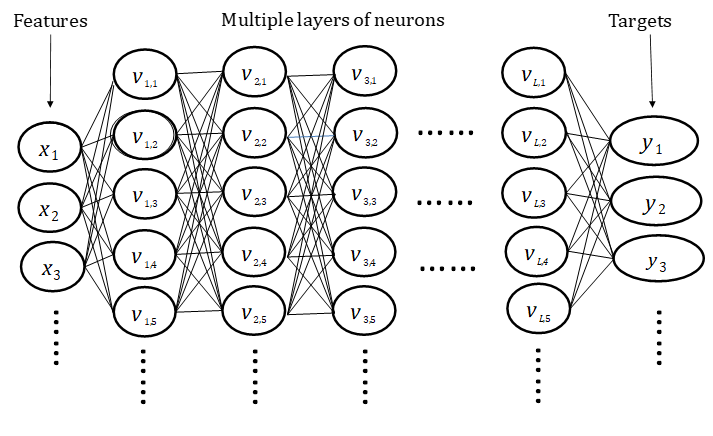
\includegraphics{./pic/chapter-5-1_pic_0.png}
\caption{caption}
\end{figure}

    Neural networks rely on \textbf{training data} to learn and improve
their accuracy over time. However, once these learning algorithms are
fine-tuned for accuracy, they are powerful tools in computer science and
artificial intelligence, allowing us to classify and cluster data at a
high velocity. Tasks in speech recognition or image recognition can take
minutes versus hours when compared to the manual identification by human
experts. One of the most well-known neural networks is Google's search
algorithm.

    \hypertarget{mc-culloch-and-pitts-artificial-neuron}{%
\subsection{Mc Culloch and Pitts Artificial
Neuron}\label{mc-culloch-and-pitts-artificial-neuron}}

    The McCulloch and Pitts neuron is one of the oldest neural network. It
has a single neuron and is the simplest form of a neural network. So it
is very important to learn how it works because it is the most
fundamental unit of a deep neural networks.

The artificial neuron receives one or more inputs and sums them to
produce an output. Usually each input is separately weighted, and the
sum is passed through a non-linear function known as an activation
function or transfer function. The transfer functions usually have a
sigmoid shape, but they may also take the form of other non-linear
functions, piecewise linear functions, or step functions. They are also
often monotonically increasing, continuous, differentiable and bounded.

    \begin{figure}
\centering
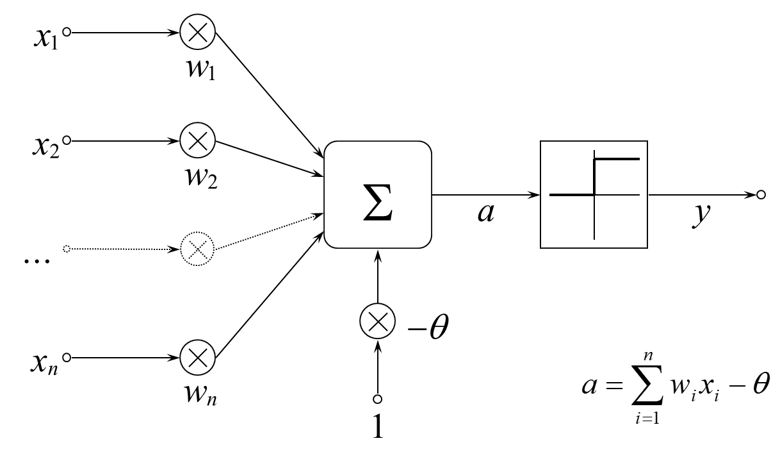
\includegraphics{./pic/chapter-5-1_pic_1.png}
\caption{caption}
\end{figure}

    \hypertarget{feedforward-neural-networks}{%
\subsection{Feedforward Neural
Networks}\label{feedforward-neural-networks}}

    Feedforward neural networks, or multi-layer perceptrons (MLPs), are what
we've primarily been focusing on within this notebook. They are
comprised of an input layer, a hidden layer or layers, and an output
layer. Data usually is fed into these models to train them, and they are
the foundation for computer vision, natural language processing, and
other neural networks.

The simplest kind of feedforward neural network is a single-layer
network, which consists of a single layer of output nodes; the inputs
are fed directly to the outputs via a series of weights. The sum of the
products of the weights and the inputs is calculated in each node, and
if the value is above some threshold the neuron fires and takes the
activated value; otherwise it takes the deactivated value.

In the following we are going to implement a very simple neural network
from scratch without any library. In my opinion this is very usefull
because most people consider neural networks as a black-box and use
libraries like Keras, TensorFlow and PyTorch which provide, among other
things, automatic differentiation without a real understanding of how a
neural network really works. Though it is not necessary to write your
own code on how to compute gradients and backprop errors, having
knowledge on it helps you in understanding a few concepts which can help
you a lot in understanding how a neural networks works..

    \hypertarget{one-hidden-layer-nn}{%
\subsubsection{One Hidden Layer NN}\label{one-hidden-layer-nn}}

We will build a shallow dense neural network with one hidden layer

    \begin{figure}
\centering
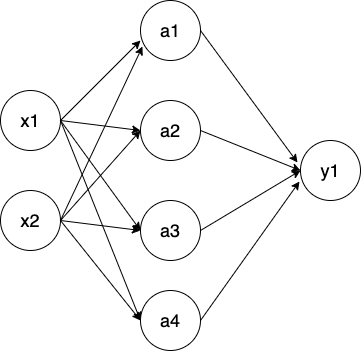
\includegraphics{./pic/chapter-5-1_pic_2.png}
\caption{caption}
\end{figure}

    Where in the graph above, we have a input vector \(x = (x_1, x_2)\),
containing 2 features and 4 hidden nodes \(a_1, a_2, a_3\) and \(a_4\),
and only one value in output \(y_1 \in [0, 1]\) (consider this a binary
classification task with a prediction of probability)

    In each hidden unit, take \(a_1\) as example, a linear operation
followed by an activation function, \(f\), is performed. So given input
\(x = (x_1, x_2)\), inside node \(a_1\), we have:

\[z_1 = w_{11}x_1 + w_{12}x_2 + b_1\]

\[a_1 = f(w_{11}x_1 + w_{12}x_2 + b_1) = f(z_1) \]

Here \(w_{11}\) denotes weight 1 of node 1, \(w_{12}\) denotes weight 2
of node 1. Same for node \(a_2\), it would have:

\[z_2 = w_{21}x_1 + w_{22}x_2 + b_2\]

\[a_2  = f(w_{21}x_1 + w_{22}x_2 + b_2) = f(z_2)\]

And same for \(a_3\) and \(a_4\) and so on \ldots{}

We can also write in a more compact form

\begin{equation}
\begin{pmatrix}
z_1 \\ z_2 \\ z_3 \\ z_4
\end{pmatrix} =
\begin{pmatrix}
w_{11} & w_{12} \\ w_{21} & w_{22} \\ w_{31} & w_{32} \\ w_{41} & w_{42}
\end{pmatrix} 
\cdot 
\begin{pmatrix}
x_1 \\ x_2 
\end{pmatrix}
+
\begin{pmatrix}
b_1 \\ b_2 \\ b_3 \\ b_4
\end{pmatrix} 
\Rightarrow Z^{[1]} = W^{[1]} \cdot X + B^{[1]} 
\end{equation}

Note that superscript \([i]\) denotes the \(ith\) layer. Let's assume
that the first activation function is the \(\tanh\) and the output
activation function is the \(sigmoid\). So the result of the hidden
layer is:

\[ A^{[1]} = \tanh{Z^{[1]}} \]

This result is applied to the output node which will perform another
linear operation with a different set of weights, \(W^{[2]}\):

\[ Z^{[2]} = W^{[2]} \cdot A^{[1]} + B^{[2]} \]

and the final output will be the result of the application of the output
node activation function (the sigmoid) to this value:

\[ \hat{y} = \sigma({Z^{[2]}})\]

For the dimension of each matrix, we have:

\begin{itemize}
\tightlist
\item
  \$ W\^{}\{{[}1{]}\}\$ in the case above would have dimension
  \(4 \times 2\), with each \(ith\) row is the weight of node \(i\)
\item
  \(B^{[1]}\) has dimension \(4 \times 1\)
\item
  \(Z^{[1]}\) and \(A^{[1]}\) both have dimention \(4 \times 1\)
\item
  \(W^{[2]}\) has dimension \(1 \times 4\)
\item
  consequently, \(Z^{[2]}\) and \(A^{[2]}\) would have dimensition
  \(1 \times 1\), which is a single value
\end{itemize}

Function \(\tanh\) and \(sigmoid\) looks as below.

    \begin{tcolorbox}[breakable, size=fbox, boxrule=1pt, pad at break*=1mm,colback=cellbackground, colframe=cellborder]
\prompt{In}{incolor}{46}{\boxspacing}
\begin{Verbatim}[commandchars=\\\{\}]
\PY{o}{\PYZpc{}}\PY{k}{matplotlib} inline

\PY{k+kn}{import} \PY{n+nn}{numpy} \PY{k}{as} \PY{n+nn}{np}
\PY{k+kn}{import} \PY{n+nn}{matplotlib}\PY{n+nn}{.}\PY{n+nn}{pyplot} \PY{k}{as} \PY{n+nn}{plt}
\end{Verbatim}
\end{tcolorbox}

    \begin{tcolorbox}[breakable, size=fbox, boxrule=1pt, pad at break*=1mm,colback=cellbackground, colframe=cellborder]
\prompt{In}{incolor}{47}{\boxspacing}
\begin{Verbatim}[commandchars=\\\{\}]
\PY{k}{def} \PY{n+nf}{tanh}\PY{p}{(}\PY{n}{x}\PY{p}{)}\PY{p}{:}
    \PY{k}{return} \PY{n}{np}\PY{o}{.}\PY{n}{tanh}\PY{p}{(}\PY{n}{x}\PY{p}{)}

\PY{k}{def} \PY{n+nf}{sigmoid}\PY{p}{(}\PY{n}{x}\PY{p}{)}\PY{p}{:}
    \PY{k}{return} \PY{l+m+mi}{1}\PY{o}{/}\PY{p}{(}\PY{l+m+mi}{1} \PY{o}{+} \PY{n}{np}\PY{o}{.}\PY{n}{exp}\PY{p}{(}\PY{o}{\PYZhy{}}\PY{n}{x}\PY{p}{)}\PY{p}{)}
\end{Verbatim}
\end{tcolorbox}

    \begin{tcolorbox}[breakable, size=fbox, boxrule=1pt, pad at break*=1mm,colback=cellbackground, colframe=cellborder]
\prompt{In}{incolor}{48}{\boxspacing}
\begin{Verbatim}[commandchars=\\\{\}]
\PY{n}{plt}\PY{o}{.}\PY{n}{figure}\PY{p}{(}\PY{n}{figsize}\PY{o}{=}\PY{p}{[}\PY{l+m+mi}{10}\PY{p}{,} \PY{l+m+mi}{4}\PY{p}{]}\PY{p}{)}
\PY{n}{x} \PY{o}{=} \PY{n}{np}\PY{o}{.}\PY{n}{linspace}\PY{p}{(}\PY{o}{\PYZhy{}}\PY{l+m+mi}{10}\PY{p}{,} \PY{l+m+mi}{10}\PY{p}{)}

\PY{n}{plt}\PY{o}{.}\PY{n}{subplot}\PY{p}{(}\PY{l+m+mi}{1}\PY{p}{,} \PY{l+m+mi}{2}\PY{p}{,} \PY{l+m+mi}{1}\PY{p}{)}
\PY{n}{plt}\PY{o}{.}\PY{n}{plot}\PY{p}{(}\PY{n}{x}\PY{p}{,} \PY{n}{sigmoid}\PY{p}{(}\PY{n}{x}\PY{p}{)}\PY{p}{)}
\PY{n}{plt}\PY{o}{.}\PY{n}{title}\PY{p}{(}\PY{l+s+s1}{\PYZsq{}}\PY{l+s+s1}{sigmoid}\PY{l+s+s1}{\PYZsq{}}\PY{p}{)}

\PY{n}{plt}\PY{o}{.}\PY{n}{subplot}\PY{p}{(}\PY{l+m+mi}{1}\PY{p}{,} \PY{l+m+mi}{2}\PY{p}{,} \PY{l+m+mi}{2}\PY{p}{)}
\PY{n}{plt}\PY{o}{.}\PY{n}{plot}\PY{p}{(}\PY{n}{x}\PY{p}{,} \PY{n}{tanh}\PY{p}{(}\PY{n}{x}\PY{p}{)}\PY{p}{)}
\PY{n}{plt}\PY{o}{.}\PY{n}{title}\PY{p}{(}\PY{l+s+s1}{\PYZsq{}}\PY{l+s+s1}{tanh}\PY{l+s+s1}{\PYZsq{}}\PY{p}{)}
\end{Verbatim}
\end{tcolorbox}

            \begin{tcolorbox}[breakable, size=fbox, boxrule=.5pt, pad at break*=1mm, opacityfill=0]
\prompt{Out}{outcolor}{48}{\boxspacing}
\begin{Verbatim}[commandchars=\\\{\}]
Text(0.5, 1.0, 'tanh')
\end{Verbatim}
\end{tcolorbox}
        
    \begin{center}
    \adjustimage{max size={0.9\linewidth}{0.9\paperheight}}{output_16_1.png}
    \end{center}
    { \hspace*{\fill} \\}
    
    Notice that the only difference of these functions is the scale of y

    \hypertarget{the-loss-function}{%
\subsubsection{The Loss Function}\label{the-loss-function}}

Remember that Linear regression uses Least Squared Error as loss
function that gives a convex graph and then we can complete the
optimization by finding its vertex as global minimum. However, it's not
an option for logistic regression anymore. Since the hypothesis is
changed, Least Squared Error will result in a non-convex graph with
local minimums by calculating with sigmoid function applied on raw model
output.

    \begin{figure}
\centering
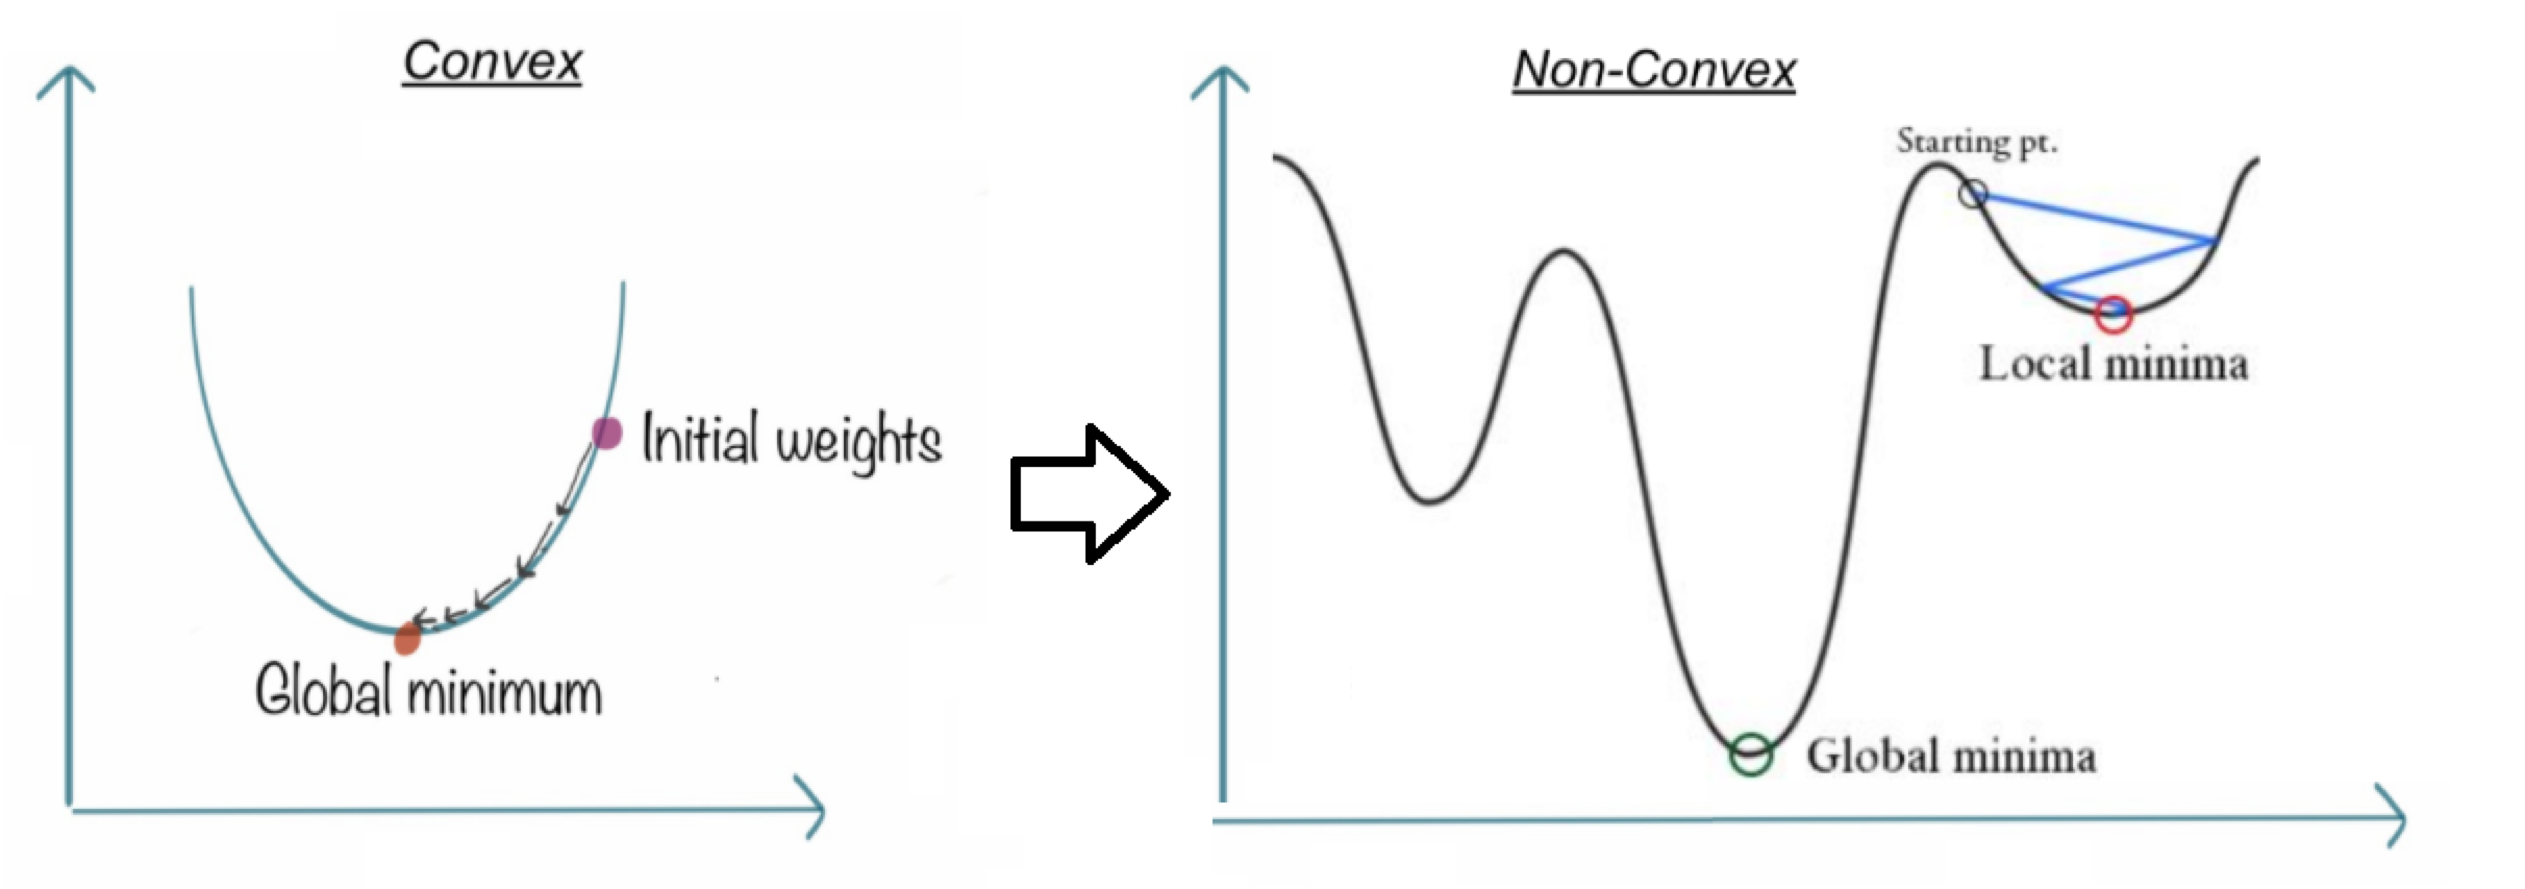
\includegraphics{./pic/chapter-5-1_pic_3.png}
\caption{caption}
\end{figure}

    Furthermore using logistic regression, means that we are focusing on
binary classification, we have class 0 and class 1. To compare with the
target, we want to constrain predictions to some values between 0 and 1.
That's why Sigmoid Function is applied on the raw model output and
provides the ability to predict with probability. So will follow a
different path.

Intuitively, we want to assign more punishment when predicting 1 while
the actual is 0 and when predict 0 while the actual is 1. The loss
function of logistic regression is doing this exactly which is called
Logistic Loss. If y = 1, when prediction = 1, the cost must be = 0,
otherwise, when prediction = 0, the learning algorithm is punished by a
very large cost. Similarly, if y = 0, predicting 0 has no punishment but
predicting 1 has a large value of cost. In formula we have

\begin{equation}
L(y, \hat{y}) = 
\begin{cases} 
-\log{\hat{y}} & \text{when}\, y = 1 \\ -\log(1 - \hat{y}) & \text{when}\, y = 0 
\end{cases} 
\end{equation}

Another advantage of this loss function is that although we are looking
at it by y = 1 and y = 0 separately, it can be written as one single
formula which brings convenience for calculation:

\[ L(y, \hat{y}) = -[y\log{\hat{y}} + (1 - y)\log{(1 - \hat{y})}] \]

    \hypertarget{formula-of-batch-training}{%
\subsubsection{Formula of Batch
Training}\label{formula-of-batch-training}}

The above shows the formula of a single input vector, however in actual
training processes, a batch is trained instead of 1 at a time. The
change applied in the formula is trivial, we just need to replace the
single vector \(x\) with a matrix \(X\) with size \(n \times m\), where
\(n\) is number of features and \(m\) is the the batch size, samples are
stacked column wise, and the following result matrix are applied
likewise. We have the same formulas as before \ldots{}

\[ Z^{[1]} = W^{[1]}X + b^{[1]}  \]

\[ A^{[1]} = \tanh{Z^{[1]}}  \]

\[ Z^{[2]} = W^{[2]}A^{[1]} + b^{[2]}  \]

\[ \hat{Y} = A^{[2]} = \sigma({Z^{[2]}})  \]

\[ J(W^{[1]}, b^{[1]}, W^{[2]}, b^{[2]}) = \frac{1}{m} \sum_{i}^{m}L(y^{(i)}, \hat{y}^{(i)})  \]

\ldots{} but for the dimension of each matrix taken in this example now
we have:

\begin{itemize}
\tightlist
\item
  \(X\) has dimension \(2 \times m\), as here there are 2 features and
  \(m\) is the batch size
\item
  \(W^{[1]}\) in the case above would have dimension \(4 \times 2\),
  with each \(ith\) row is the weight of node \(i\)
\item
  \(b^{[1]}\) has dimension \(4 \times 1\)
\item
  \(Z^{[1]}\) and \(A^{[1]}\) both have dimension \(4 \times m\)
\item
  \(W^{[2]}\) has dimension \(1 \times 4\)
\item
  consequently, \(Z^{[2]}\) and \(A^{[2]}\) would have dimension
  \(1 \times m\)
\end{itemize}

Also the loss function is the same as logistic regression, but for batch
training, we'll take the average loss for all training samples.

This is all for the forward propagation. To activate our neurons to
learn, we need to get derivative of weight parameters and update them
use gradient descent.

But now it is enough for us to implement the forward propagation first.

    \hypertarget{generate-sample-dataset}{%
\subsubsection{Generate Sample Dataset}\label{generate-sample-dataset}}

Scikit-learn includes various random sample generators that can be used
to build artificial datasets of controlled size and complexity. Here we
generate a simple \textbf{binary classification task} with 5000 data
points and 20 features for later model validation.

    \begin{tcolorbox}[breakable, size=fbox, boxrule=1pt, pad at break*=1mm,colback=cellbackground, colframe=cellborder]
\prompt{In}{incolor}{49}{\boxspacing}
\begin{Verbatim}[commandchars=\\\{\}]
\PY{k+kn}{from} \PY{n+nn}{sklearn} \PY{k+kn}{import} \PY{n}{datasets}

\PY{c+c1}{\PYZsh{} Signature of make\PYZus{}classification}
\PY{c+c1}{\PYZsh{} }
\PY{c+c1}{\PYZsh{} make\PYZus{}classification (}
\PY{c+c1}{\PYZsh{} n\PYZus{}samples: int=100,}
\PY{c+c1}{\PYZsh{} n\PYZus{}features: int=20,}
\PY{c+c1}{\PYZsh{} n\PYZus{}informative: int=2,}
\PY{c+c1}{\PYZsh{} n\PYZus{}redundant: int=2,}
\PY{c+c1}{\PYZsh{} n\PYZus{}repeated: int=0,}
\PY{c+c1}{\PYZsh{} n\PYZus{}classes: int=2,}
\PY{c+c1}{\PYZsh{} n\PYZus{}clusters\PYZus{}per\PYZus{}class: int=2,}
\PY{c+c1}{\PYZsh{} weights: \PYZus{}\PYZus{}class\PYZus{}\PYZus{}=None,}
\PY{c+c1}{\PYZsh{} flip\PYZus{}y: float=0.01,}
\PY{c+c1}{\PYZsh{} class\PYZus{}sep: float=1,}
\PY{c+c1}{\PYZsh{} hypercube: bool=True,}
\PY{c+c1}{\PYZsh{} shift: float=0,}
\PY{c+c1}{\PYZsh{} scale: float=1,}
\PY{c+c1}{\PYZsh{} shuffle: bool=True,}
\PY{c+c1}{\PYZsh{} random\PYZus{}state: \PYZus{}\PYZus{}class\PYZus{}\PYZus{}=None}
\PY{c+c1}{\PYZsh{} )}

\PY{n}{X}\PY{p}{,} \PY{n}{y} \PY{o}{=} \PY{n}{datasets}\PY{o}{.}\PY{n}{make\PYZus{}classification}\PY{p}{(}\PY{n}{n\PYZus{}samples}\PY{o}{=}\PY{l+m+mi}{5000}\PY{p}{,} \PY{n}{random\PYZus{}state}\PY{o}{=}\PY{l+m+mi}{123}\PY{p}{)}

\PY{n}{X\PYZus{}train}\PY{p}{,} \PY{n}{X\PYZus{}test} \PY{o}{=} \PY{n}{X}\PY{p}{[}\PY{p}{:}\PY{l+m+mi}{4000}\PY{p}{]}\PY{p}{,} \PY{n}{X}\PY{p}{[}\PY{l+m+mi}{4000}\PY{p}{:}\PY{p}{]}
\PY{n}{y\PYZus{}train}\PY{p}{,} \PY{n}{y\PYZus{}test} \PY{o}{=} \PY{n}{y}\PY{p}{[}\PY{p}{:}\PY{l+m+mi}{4000}\PY{p}{]}\PY{p}{,} \PY{n}{y}\PY{p}{[}\PY{l+m+mi}{4000}\PY{p}{:}\PY{p}{]}

\PY{n+nb}{print}\PY{p}{(}\PY{l+s+s1}{\PYZsq{}}\PY{l+s+s1}{train shape}\PY{l+s+s1}{\PYZsq{}}\PY{p}{,} \PY{n}{X\PYZus{}train}\PY{o}{.}\PY{n}{shape}\PY{p}{)}
\PY{n+nb}{print}\PY{p}{(}\PY{l+s+s1}{\PYZsq{}}\PY{l+s+s1}{test shape}\PY{l+s+s1}{\PYZsq{}}\PY{p}{,} \PY{n}{X\PYZus{}test}\PY{o}{.}\PY{n}{shape}\PY{p}{)}
\end{Verbatim}
\end{tcolorbox}

    \begin{Verbatim}[commandchars=\\\{\}]
train shape (4000, 20)
test shape (1000, 20)
    \end{Verbatim}

    \begin{tcolorbox}[breakable, size=fbox, boxrule=1pt, pad at break*=1mm,colback=cellbackground, colframe=cellborder]
\prompt{In}{incolor}{50}{\boxspacing}
\begin{Verbatim}[commandchars=\\\{\}]
\PY{n+nb}{print}\PY{p}{(}\PY{n}{X}\PY{p}{[}\PY{l+m+mi}{0}\PY{p}{]}\PY{p}{)}
\end{Verbatim}
\end{tcolorbox}

    \begin{Verbatim}[commandchars=\\\{\}]
[ 0.72613439 -0.09447897 -0.40795222  0.89879088  0.10474933 -1.66342926
 -0.72927498  0.10438512  1.56349884  0.28581615  1.15799916 -0.15592708
  0.82470152 -1.19743807  0.68883271 -1.50530988  0.93842871  0.38021827
 -0.66238809  0.43334625]
    \end{Verbatim}

    \begin{tcolorbox}[breakable, size=fbox, boxrule=1pt, pad at break*=1mm,colback=cellbackground, colframe=cellborder]
\prompt{In}{incolor}{51}{\boxspacing}
\begin{Verbatim}[commandchars=\\\{\}]
\PY{n+nb}{print}\PY{p}{(}\PY{n}{y}\PY{p}{[}\PY{l+m+mi}{0}\PY{p}{]}\PY{p}{)}
\end{Verbatim}
\end{tcolorbox}

    \begin{Verbatim}[commandchars=\\\{\}]
1
    \end{Verbatim}

    \begin{tcolorbox}[breakable, size=fbox, boxrule=1pt, pad at break*=1mm,colback=cellbackground, colframe=cellborder]
\prompt{In}{incolor}{52}{\boxspacing}
\begin{Verbatim}[commandchars=\\\{\}]
\PY{c+c1}{\PYZsh{}plt.scatter(X[:, 0], X[:, 1], marker=\PYZsq{}o\PYZsq{}, c=y,s=25, edgecolor=\PYZsq{}k\PYZsq{})}
\end{Verbatim}
\end{tcolorbox}

    \hypertarget{weights-initialization}{%
\subsubsection{Weights Initialization}\label{weights-initialization}}

Our neural network has 1 hidden layer and 2 layers in total(hidden layer
+ output layer), so there are 4 weight matrices to initialize
(\(W^{[1]}, b^{[1]}\) and \(W^{[2]}, b^{[2]}\)). Notice that the weights
are initialized relatively small so that the gradients would be higher
thus learning faster in the beginning phase.

    \begin{tcolorbox}[breakable, size=fbox, boxrule=1pt, pad at break*=1mm,colback=cellbackground, colframe=cellborder]
\prompt{In}{incolor}{53}{\boxspacing}
\begin{Verbatim}[commandchars=\\\{\}]
\PY{k}{def} \PY{n+nf}{init\PYZus{}weights}\PY{p}{(}\PY{n}{n\PYZus{}input}\PY{p}{,} \PY{n}{n\PYZus{}hidden}\PY{p}{,} \PY{n}{n\PYZus{}output}\PY{p}{)}\PY{p}{:}
    \PY{n}{params} \PY{o}{=} \PY{p}{\PYZob{}}\PY{p}{\PYZcb{}}
    \PY{n}{params}\PY{p}{[}\PY{l+s+s1}{\PYZsq{}}\PY{l+s+s1}{W1}\PY{l+s+s1}{\PYZsq{}}\PY{p}{]} \PY{o}{=} \PY{n}{np}\PY{o}{.}\PY{n}{random}\PY{o}{.}\PY{n}{randn}\PY{p}{(}\PY{n}{n\PYZus{}hidden}\PY{p}{,} \PY{n}{n\PYZus{}input}\PY{p}{)} \PY{o}{*} \PY{l+m+mf}{0.01}
    \PY{n}{params}\PY{p}{[}\PY{l+s+s1}{\PYZsq{}}\PY{l+s+s1}{b1}\PY{l+s+s1}{\PYZsq{}}\PY{p}{]} \PY{o}{=} \PY{n}{np}\PY{o}{.}\PY{n}{zeros}\PY{p}{(}\PY{p}{(}\PY{n}{n\PYZus{}hidden}\PY{p}{,} \PY{l+m+mi}{1}\PY{p}{)}\PY{p}{)}
    \PY{n}{params}\PY{p}{[}\PY{l+s+s1}{\PYZsq{}}\PY{l+s+s1}{W2}\PY{l+s+s1}{\PYZsq{}}\PY{p}{]} \PY{o}{=} \PY{n}{np}\PY{o}{.}\PY{n}{random}\PY{o}{.}\PY{n}{randn}\PY{p}{(}\PY{n}{n\PYZus{}output}\PY{p}{,} \PY{n}{n\PYZus{}hidden}\PY{p}{)} \PY{o}{*} \PY{l+m+mf}{0.01}
    \PY{n}{params}\PY{p}{[}\PY{l+s+s1}{\PYZsq{}}\PY{l+s+s1}{b2}\PY{l+s+s1}{\PYZsq{}}\PY{p}{]} \PY{o}{=} \PY{n}{np}\PY{o}{.}\PY{n}{zeros}\PY{p}{(}\PY{p}{(}\PY{n}{n\PYZus{}output}\PY{p}{,} \PY{l+m+mi}{1}\PY{p}{)}\PY{p}{)}
    
    \PY{k}{return} \PY{n}{params}
\end{Verbatim}
\end{tcolorbox}

    \begin{tcolorbox}[breakable, size=fbox, boxrule=1pt, pad at break*=1mm,colback=cellbackground, colframe=cellborder]
\prompt{In}{incolor}{54}{\boxspacing}
\begin{Verbatim}[commandchars=\\\{\}]
\PY{n}{params} \PY{o}{=} \PY{n}{init\PYZus{}weights}\PY{p}{(}\PY{l+m+mi}{20}\PY{p}{,} \PY{l+m+mi}{10}\PY{p}{,} \PY{l+m+mi}{1}\PY{p}{)}

\PY{n+nb}{print}\PY{p}{(}\PY{l+s+s1}{\PYZsq{}}\PY{l+s+s1}{W1 shape}\PY{l+s+s1}{\PYZsq{}}\PY{p}{,} \PY{n}{params}\PY{p}{[}\PY{l+s+s1}{\PYZsq{}}\PY{l+s+s1}{W1}\PY{l+s+s1}{\PYZsq{}}\PY{p}{]}\PY{o}{.}\PY{n}{shape}\PY{p}{)}
\PY{n+nb}{print}\PY{p}{(}\PY{l+s+s1}{\PYZsq{}}\PY{l+s+s1}{b1 shape}\PY{l+s+s1}{\PYZsq{}}\PY{p}{,} \PY{n}{params}\PY{p}{[}\PY{l+s+s1}{\PYZsq{}}\PY{l+s+s1}{b1}\PY{l+s+s1}{\PYZsq{}}\PY{p}{]}\PY{o}{.}\PY{n}{shape}\PY{p}{)}
\PY{n+nb}{print}\PY{p}{(}\PY{l+s+s1}{\PYZsq{}}\PY{l+s+s1}{W2 shape}\PY{l+s+s1}{\PYZsq{}}\PY{p}{,} \PY{n}{params}\PY{p}{[}\PY{l+s+s1}{\PYZsq{}}\PY{l+s+s1}{W2}\PY{l+s+s1}{\PYZsq{}}\PY{p}{]}\PY{o}{.}\PY{n}{shape}\PY{p}{)}
\PY{n+nb}{print}\PY{p}{(}\PY{l+s+s1}{\PYZsq{}}\PY{l+s+s1}{b2 shape}\PY{l+s+s1}{\PYZsq{}}\PY{p}{,} \PY{n}{params}\PY{p}{[}\PY{l+s+s1}{\PYZsq{}}\PY{l+s+s1}{b2}\PY{l+s+s1}{\PYZsq{}}\PY{p}{]}\PY{o}{.}\PY{n}{shape}\PY{p}{)}
\end{Verbatim}
\end{tcolorbox}

    \begin{Verbatim}[commandchars=\\\{\}]
W1 shape (10, 20)
b1 shape (10, 1)
W2 shape (1, 10)
b2 shape (1, 1)
    \end{Verbatim}

    \hypertarget{forward-propagation}{%
\subsubsection{Forward Propagation}\label{forward-propagation}}

Let's implement the forward process following equations
\((5) \sim (8)\).

    \begin{tcolorbox}[breakable, size=fbox, boxrule=1pt, pad at break*=1mm,colback=cellbackground, colframe=cellborder]
\prompt{In}{incolor}{55}{\boxspacing}
\begin{Verbatim}[commandchars=\\\{\}]
\PY{k}{def} \PY{n+nf}{forward}\PY{p}{(}\PY{n}{X}\PY{p}{,} \PY{n}{params}\PY{p}{)}\PY{p}{:}
    \PY{l+s+sd}{\PYZdq{}\PYZdq{}\PYZdq{}}
\PY{l+s+sd}{    X: need to have shape (n\PYZus{}features x m\PYZus{}samples)}
\PY{l+s+sd}{    \PYZdq{}\PYZdq{}\PYZdq{}}
    \PY{n}{W1}\PY{p}{,} \PY{n}{b1}\PY{p}{,} \PY{n}{W2}\PY{p}{,} \PY{n}{b2} \PY{o}{=} \PY{n}{params}\PY{p}{[}\PY{l+s+s1}{\PYZsq{}}\PY{l+s+s1}{W1}\PY{l+s+s1}{\PYZsq{}}\PY{p}{]}\PY{p}{,} \PY{n}{params}\PY{p}{[}\PY{l+s+s1}{\PYZsq{}}\PY{l+s+s1}{b1}\PY{l+s+s1}{\PYZsq{}}\PY{p}{]}\PY{p}{,} \PY{n}{params}\PY{p}{[}\PY{l+s+s1}{\PYZsq{}}\PY{l+s+s1}{W2}\PY{l+s+s1}{\PYZsq{}}\PY{p}{]}\PY{p}{,} \PY{n}{params}\PY{p}{[}\PY{l+s+s1}{\PYZsq{}}\PY{l+s+s1}{b2}\PY{l+s+s1}{\PYZsq{}}\PY{p}{]}
    \PY{n}{A0} \PY{o}{=} \PY{n}{X}
    
    \PY{n}{cache} \PY{o}{=} \PY{p}{\PYZob{}}\PY{p}{\PYZcb{}}
    \PY{n}{Z1} \PY{o}{=} \PY{n}{np}\PY{o}{.}\PY{n}{dot}\PY{p}{(}\PY{n}{W1}\PY{p}{,} \PY{n}{A0}\PY{p}{)} \PY{o}{+} \PY{n}{b1}
    \PY{n}{A1} \PY{o}{=} \PY{n}{tanh}\PY{p}{(}\PY{n}{Z1}\PY{p}{)}
    \PY{n}{Z2} \PY{o}{=} \PY{n}{np}\PY{o}{.}\PY{n}{dot}\PY{p}{(}\PY{n}{W2}\PY{p}{,} \PY{n}{A1}\PY{p}{)} \PY{o}{+} \PY{n}{b2}
    \PY{n}{A2} \PY{o}{=} \PY{n}{sigmoid}\PY{p}{(}\PY{n}{Z2}\PY{p}{)}
    
    \PY{n}{cache}\PY{p}{[}\PY{l+s+s1}{\PYZsq{}}\PY{l+s+s1}{Z1}\PY{l+s+s1}{\PYZsq{}}\PY{p}{]} \PY{o}{=} \PY{n}{Z1}
    \PY{n}{cache}\PY{p}{[}\PY{l+s+s1}{\PYZsq{}}\PY{l+s+s1}{A1}\PY{l+s+s1}{\PYZsq{}}\PY{p}{]} \PY{o}{=} \PY{n}{A1}
    \PY{n}{cache}\PY{p}{[}\PY{l+s+s1}{\PYZsq{}}\PY{l+s+s1}{Z2}\PY{l+s+s1}{\PYZsq{}}\PY{p}{]} \PY{o}{=} \PY{n}{Z2}
    \PY{n}{cache}\PY{p}{[}\PY{l+s+s1}{\PYZsq{}}\PY{l+s+s1}{A2}\PY{l+s+s1}{\PYZsq{}}\PY{p}{]} \PY{o}{=} \PY{n}{A2}
    \PY{k}{return}  \PY{n}{cache}
\end{Verbatim}
\end{tcolorbox}

    \begin{tcolorbox}[breakable, size=fbox, boxrule=1pt, pad at break*=1mm,colback=cellbackground, colframe=cellborder]
\prompt{In}{incolor}{56}{\boxspacing}
\begin{Verbatim}[commandchars=\\\{\}]
\PY{c+c1}{\PYZsh{} get 100 samples}
\PY{n}{inp} \PY{o}{=} \PY{n}{X}\PY{p}{[}\PY{p}{:}\PY{l+m+mi}{100}\PY{p}{]}\PY{o}{.}\PY{n}{T}

\PY{n}{cache} \PY{o}{=} \PY{n}{forward}\PY{p}{(}\PY{n}{inp}\PY{p}{,} \PY{n}{params}\PY{p}{)}

\PY{n+nb}{print}\PY{p}{(}\PY{l+s+s1}{\PYZsq{}}\PY{l+s+s1}{Z1 shape}\PY{l+s+s1}{\PYZsq{}}\PY{p}{,} \PY{n}{cache}\PY{p}{[}\PY{l+s+s1}{\PYZsq{}}\PY{l+s+s1}{Z1}\PY{l+s+s1}{\PYZsq{}}\PY{p}{]}\PY{o}{.}\PY{n}{shape}\PY{p}{)}
\PY{n+nb}{print}\PY{p}{(}\PY{l+s+s1}{\PYZsq{}}\PY{l+s+s1}{A1 shape}\PY{l+s+s1}{\PYZsq{}}\PY{p}{,} \PY{n}{cache}\PY{p}{[}\PY{l+s+s1}{\PYZsq{}}\PY{l+s+s1}{A1}\PY{l+s+s1}{\PYZsq{}}\PY{p}{]}\PY{o}{.}\PY{n}{shape}\PY{p}{)}
\PY{n+nb}{print}\PY{p}{(}\PY{l+s+s1}{\PYZsq{}}\PY{l+s+s1}{Z2 shape}\PY{l+s+s1}{\PYZsq{}}\PY{p}{,} \PY{n}{cache}\PY{p}{[}\PY{l+s+s1}{\PYZsq{}}\PY{l+s+s1}{Z2}\PY{l+s+s1}{\PYZsq{}}\PY{p}{]}\PY{o}{.}\PY{n}{shape}\PY{p}{)}
\PY{n+nb}{print}\PY{p}{(}\PY{l+s+s1}{\PYZsq{}}\PY{l+s+s1}{A2 shape}\PY{l+s+s1}{\PYZsq{}}\PY{p}{,} \PY{n}{cache}\PY{p}{[}\PY{l+s+s1}{\PYZsq{}}\PY{l+s+s1}{A2}\PY{l+s+s1}{\PYZsq{}}\PY{p}{]}\PY{o}{.}\PY{n}{shape}\PY{p}{)}
\end{Verbatim}
\end{tcolorbox}

    \begin{Verbatim}[commandchars=\\\{\}]
Z1 shape (10, 100)
A1 shape (10, 100)
Z2 shape (1, 100)
A2 shape (1, 100)
    \end{Verbatim}

    \hypertarget{loss-function}{%
\subsubsection{Loss Function}\label{loss-function}}

Following equation \((9)\), let's calculate the loss of each batch.

    \begin{tcolorbox}[breakable, size=fbox, boxrule=1pt, pad at break*=1mm,colback=cellbackground, colframe=cellborder]
\prompt{In}{incolor}{57}{\boxspacing}
\begin{Verbatim}[commandchars=\\\{\}]
\PY{k}{def} \PY{n+nf}{loss}\PY{p}{(}\PY{n}{Y}\PY{p}{,} \PY{n}{Y\PYZus{}hat}\PY{p}{)}\PY{p}{:}
    \PY{l+s+sd}{\PYZdq{}\PYZdq{}\PYZdq{}}
\PY{l+s+sd}{    Y: vector of true value}
\PY{l+s+sd}{    Y\PYZus{}hat: vector of predicted value}
\PY{l+s+sd}{    \PYZdq{}\PYZdq{}\PYZdq{}}
    \PY{k}{assert} \PY{n}{Y}\PY{o}{.}\PY{n}{shape}\PY{p}{[}\PY{l+m+mi}{0}\PY{p}{]} \PY{o}{==} \PY{l+m+mi}{1}
    \PY{k}{assert} \PY{n}{Y}\PY{o}{.}\PY{n}{shape} \PY{o}{==} \PY{n}{Y\PYZus{}hat}\PY{o}{.}\PY{n}{shape}
    \PY{n}{m} \PY{o}{=} \PY{n}{Y}\PY{o}{.}\PY{n}{shape}\PY{p}{[}\PY{l+m+mi}{1}\PY{p}{]}
    \PY{n}{s} \PY{o}{=} \PY{n}{Y} \PY{o}{*} \PY{n}{np}\PY{o}{.}\PY{n}{log}\PY{p}{(}\PY{n}{Y\PYZus{}hat}\PY{p}{)} \PY{o}{+} \PY{p}{(}\PY{l+m+mi}{1} \PY{o}{\PYZhy{}} \PY{n}{Y}\PY{p}{)} \PY{o}{*} \PY{n}{np}\PY{o}{.}\PY{n}{log}\PY{p}{(}\PY{l+m+mi}{1} \PY{o}{\PYZhy{}} \PY{n}{Y\PYZus{}hat}\PY{p}{)}
    \PY{n}{loss} \PY{o}{=} \PY{o}{\PYZhy{}}\PY{n}{np}\PY{o}{.}\PY{n}{sum}\PY{p}{(}\PY{n}{s}\PY{p}{)} \PY{o}{/} \PY{n}{m}
    \PY{k}{return} \PY{n}{loss}
\end{Verbatim}
\end{tcolorbox}

    \begin{tcolorbox}[breakable, size=fbox, boxrule=1pt, pad at break*=1mm,colback=cellbackground, colframe=cellborder]
\prompt{In}{incolor}{58}{\boxspacing}
\begin{Verbatim}[commandchars=\\\{\}]
\PY{n}{Y} \PY{o}{=} \PY{n}{np}\PY{o}{.}\PY{n}{array}\PY{p}{(}\PY{p}{[}\PY{n}{np}\PY{o}{.}\PY{n}{random}\PY{o}{.}\PY{n}{choice}\PY{p}{(}\PY{p}{[}\PY{l+m+mi}{0}\PY{p}{,} \PY{l+m+mi}{1}\PY{p}{]}\PY{p}{)} \PY{k}{for} \PY{n}{i} \PY{o+ow}{in} \PY{n+nb}{range}\PY{p}{(}\PY{l+m+mi}{10}\PY{p}{)}\PY{p}{]}\PY{p}{)}\PY{o}{.}\PY{n}{reshape}\PY{p}{(}\PY{l+m+mi}{1}\PY{p}{,} \PY{o}{\PYZhy{}}\PY{l+m+mi}{1}\PY{p}{)}
\PY{n}{Y\PYZus{}hat} \PY{o}{=} \PY{n}{np}\PY{o}{.}\PY{n}{random}\PY{o}{.}\PY{n}{uniform}\PY{p}{(}\PY{l+m+mi}{0}\PY{p}{,} \PY{l+m+mi}{1}\PY{p}{,} \PY{l+m+mi}{10}\PY{p}{)}\PY{o}{.}\PY{n}{reshape}\PY{p}{(}\PY{l+m+mi}{1}\PY{p}{,} \PY{o}{\PYZhy{}}\PY{l+m+mi}{1}\PY{p}{)}

\PY{n}{l} \PY{o}{=} \PY{n}{loss}\PY{p}{(}\PY{n}{Y}\PY{p}{,} \PY{n}{Y\PYZus{}hat}\PY{p}{)}
\PY{n+nb}{print}\PY{p}{(}\PY{l+s+sa}{f}\PY{l+s+s1}{\PYZsq{}}\PY{l+s+s1}{loss }\PY{l+s+si}{\PYZob{}}\PY{n}{l}\PY{l+s+si}{\PYZcb{}}\PY{l+s+s1}{\PYZsq{}}\PY{p}{)}
\end{Verbatim}
\end{tcolorbox}

    \begin{Verbatim}[commandchars=\\\{\}]
loss 1.1942297105295607
    \end{Verbatim}

    \hypertarget{delta-rule}{%
\subsubsection{Delta Rule}\label{delta-rule}}

Now it comes to the so colled \textbf{\emph{delta rule}} which is the
key to our weights update. With \emph{delta rule} we compute the
gradient of the loss function with respect to the weights of the network
for a single input--output example.

Given a generic actual value \(y\), we want to minimize the loss \(L\),
and the technic we are going to apply here is gradient descent,
basically what we need to do is to apply derivative to our variables and
move them slightly down to the optimum. Here we have 2 variables, \(W\)
and \(b\), and for this example, the update formula of them would be:

\[W = W - \frac{\partial L}{\partial W}\]

\[b = b - \frac{\partial L}{\partial b}\]

The delta rule algorithm works by computing the gradient of the loss
function with respect to each weight. In order to get the derivative of
our targets, chain rules would be applied:

\[\frac{\partial L}{\partial W} =  \frac{\partial L}{\partial \hat y} \frac{\partial \hat y}{\partial Z} \frac{\partial Z}{\partial W} \]

\[\frac{\partial L}{\partial b} =  \frac{\partial L}{\partial \hat y} \frac{\partial \hat y}{\partial Z} \frac{\partial Z}{\partial b} \]

Let's calculate \ldots{}

\hypertarget{gradient-calculation}{%
\paragraph{Gradient Calculation}\label{gradient-calculation}}

\[L(y, \hat{y}) = -[y\log{\hat{y}} + (1 - y)\log{(1 - \hat{y})}] \Rightarrow 
\frac{\partial L}{\partial \hat y} = -\frac{y}{\hat y} + \frac{1-y}{1-\hat y} = \frac{\hat y - y}{\hat y(1 - \hat y)}\]

\[ Z = W^{[i]} \cdot x^{[i]} + B^{[i]} \Rightarrow \frac{\partial Z}{\partial W} = x \quad \frac{\partial Z}{\partial b} = 1\]

We have to compute the derivatives of the activation functions (see
appendix for details):

\textbf{Hidden Layer Activation Function (Hyperbolic Tangent)}

\begin{equation}
\tanh x = \frac{{{e^x} – {e^{ – x}}}}{{{e^x} + {e^{ – x}}}} 
\Rightarrow 
\frac{d}{{dx}}\tanh x =  1 - {\left(\tanh x \right)}^2 
\end{equation}

\textbf{Output Layer Activation Function (Sigmoid Function)}

\begin{equation}
\sigma(x) =  \left[ \dfrac{1}{1 + e^{-x}} \right]  \Rightarrow
\dfrac{d}{dx} \sigma(x) =  \sigma(x) \cdot (1 - \sigma(x))
\end{equation}

Given the loss function \(L\) we defined above, we have gradients as
follows:

\textbf{Output Layer}

\begin{align}
& \frac{\partial L}{\partial \hat y} = \frac{\hat y - y}{\hat y(1 - \hat y)} \notag\\
& \frac{\partial Z}{\partial W_O} = x \notag\\
& \frac{\partial \hat y}{\partial Z} = \frac{\partial \sigma}{\partial Z} = \sigma(Z) \cdot (1 - \sigma(Z)) = (\hat y) (1 - \hat y)
\end{align}

So the complete gradient is:

\begin{align}
& \frac{\partial L}{\partial W_O} =  \frac{\partial L}{\partial \hat y} \frac{\partial \hat y}{\partial Z} \frac{\partial Z}{\partial W_O} = (\hat y - y) \cdot x \notag\\
& \frac{\partial L}{\partial b} =  (\hat y - y)
\end{align}

\textbf{Hidden Layer}

Now we have to calculate

\[\frac{\partial Z}{\partial W_H}\]

Remember that

\[Z = W_O \cdot tanh\left( W_H \cdot X + b_H \right) + b_O\]

and

\[\frac{\partial Z}{\partial W_H} = W_O \cdot \frac{\partial \, tanh(\dots)}{\partial W_H} \cdot X = W_O \cdot \left( 1 - tanh^2(\dots) \right) \cdot X\]

and finally

\begin{equation}
\frac{\partial L}{\partial W_H} = (\hat y - y) \cdot W_O \cdot X \cdot \left( 1 - tanh^2(\dots) \right)
\end{equation}

\hypertarget{weights-update}{%
\paragraph{Weights Update}\label{weights-update}}

Now we can compute changes in weight matrices

\textbf{Output Layer}

\begin{align}
& dW^{[2]} = \frac{1}{m}\left[A^{[2]} - Y \right]A^{[1]^T} = \frac{1}{m}\Delta^{[2]}A^{[1]^T} \\
& db^{[2]} = \frac{1}{m}np.sum(dZ^{[2]}, axis=1, keepdims=True) 
\end{align}

\textbf{Hidden Layer}

\begin{align}
dW^{[1]} &= \frac{1}{m} \left[ A^{[2]} - Y \right] \cdot  X^{T} \cdot W^{[2]T} \cdot (1 - A^{[1]^2}) \notag\\
         &= \frac{1}{m} \Delta^{[2]} \cdot W^{[2]T} \cdot (1 - A^{[1]^2}) \cdot  X^{T}   \notag\\
         &= \frac{1}{m} \Delta^{[1]} \cdot  X^{T} 
\end{align}

\begin{equation} 
db^{[1]} = \frac{1}{m}np.sum(dZ^{[1]}, axis=1, keepdims=True)  
\end{equation}

where

\begin{align} 
& \Delta^{[2]} = A^{[2]} - Y  \\
& \Delta^{[1]} = \Delta^{[2]} \cdot W^{[2]T} \cdot (1 - A^{[1]^2})
\end{align}

In summary:

\begin{itemize}
\tightlist
\item
  Error is calculated between the expected outputs and the outputs
  forward propagated from the network.
\item
  These errors are then propagated backward through the network from the
  output layer to the hidden layer, assigning a penalty for the error
  and updating weights as they go.
\end{itemize}

    \begin{figure}
\centering
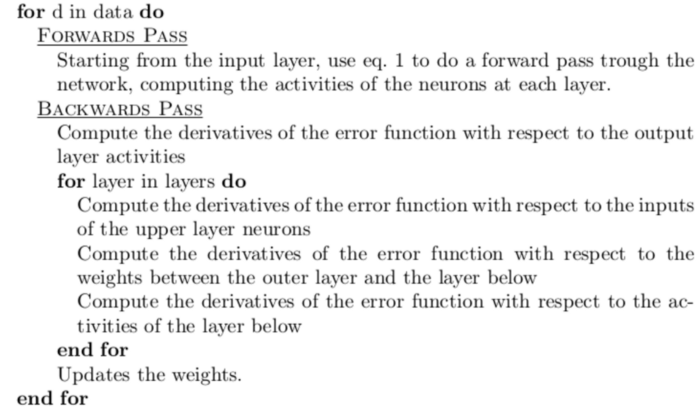
\includegraphics{./pic/chapter-5-1_pic_4.png}
\caption{caption}
\end{figure}

    In equation \((4)\) is element-wise multiplication, and the gradient of
\(\tanh{x}\) is \(1 - x^2\). You can try to deduct the equation above by
yourself, but I basically took it from internet.

Let's break down the shape of each element, given number of each layer
equals \texttt{(n\_x,\ n\_h,\ n\_y)} and batch size equals \texttt{m}:

\begin{itemize}
\item
  \(A^{[2]}\), \(Y\) and \(dZ^{[2]}\) has shape \texttt{(n\_y,\ m)}
\item
  Because \(A^{[1]}\) has shape \texttt{(n\_h,\ m)}, \(dW^{[2]}\) would
  have shape \texttt{(n\_y,\ n\_h)}
\item
  \(db^{[2]}\) has shape \texttt{(n\_y,\ 1)}
\item
  Because \(dZ^{[2]}\) has shape \texttt{(n\_y,\ m)}, \(W^{[2]}\) has
  shape\texttt{(n\_y,\ n\_h)}, \(dZ^{[1]}\) would have shape
  \texttt{(n\_h,\ m)}
\item
  In equation \((5)\), \(X\) has shape \texttt{(n\_x,\ m)}, so
  \(dW^{[1]}\) has shape \texttt{(n\_h,\ n\_x)}
\item
  \(db^{[1]}\) has shape \texttt{(n\_h,\ 1)}
\end{itemize}

Once we understand the formula, implementation should come with ease.

    \begin{tcolorbox}[breakable, size=fbox, boxrule=1pt, pad at break*=1mm,colback=cellbackground, colframe=cellborder]
\prompt{In}{incolor}{59}{\boxspacing}
\begin{Verbatim}[commandchars=\\\{\}]
\PY{k}{def} \PY{n+nf}{backward}\PY{p}{(}\PY{n}{params}\PY{p}{,} \PY{n}{cache}\PY{p}{,} \PY{n}{X}\PY{p}{,} \PY{n}{Y}\PY{p}{)}\PY{p}{:}
    \PY{l+s+sd}{\PYZdq{}\PYZdq{}\PYZdq{}}
\PY{l+s+sd}{    [From coursera deep\PYZhy{}learning course]}
\PY{l+s+sd}{    params: we initiate above with W1, b1, W2, b2}
\PY{l+s+sd}{    cache: the intermediate caculation we saved with Z1, A1, Z2, A2}
\PY{l+s+sd}{    X: shape of (n\PYZus{}x, m)}
\PY{l+s+sd}{    Y: shape (n\PYZus{}y, m)}
\PY{l+s+sd}{    \PYZdq{}\PYZdq{}\PYZdq{}}
    
    \PY{n}{m} \PY{o}{=} \PY{n}{X}\PY{o}{.}\PY{n}{shape}\PY{p}{[}\PY{l+m+mi}{1}\PY{p}{]}

    \PY{n}{W1} \PY{o}{=} \PY{n}{params}\PY{p}{[}\PY{l+s+s1}{\PYZsq{}}\PY{l+s+s1}{W1}\PY{l+s+s1}{\PYZsq{}}\PY{p}{]}
    \PY{n}{W2} \PY{o}{=} \PY{n}{params}\PY{p}{[}\PY{l+s+s1}{\PYZsq{}}\PY{l+s+s1}{W2}\PY{l+s+s1}{\PYZsq{}}\PY{p}{]}
    \PY{n}{A1} \PY{o}{=} \PY{n}{cache}\PY{p}{[}\PY{l+s+s1}{\PYZsq{}}\PY{l+s+s1}{A1}\PY{l+s+s1}{\PYZsq{}}\PY{p}{]}
    \PY{n}{A2} \PY{o}{=} \PY{n}{cache}\PY{p}{[}\PY{l+s+s1}{\PYZsq{}}\PY{l+s+s1}{A2}\PY{l+s+s1}{\PYZsq{}}\PY{p}{]}

    \PY{n}{DL2} \PY{o}{=} \PY{n}{A2} \PY{o}{\PYZhy{}} \PY{n}{Y}
    \PY{n}{dW2} \PY{o}{=} \PY{p}{(}\PY{l+m+mi}{1} \PY{o}{/} \PY{n}{m}\PY{p}{)} \PY{o}{*} \PY{n}{np}\PY{o}{.}\PY{n}{dot}\PY{p}{(}\PY{n}{DL2}\PY{p}{,} \PY{n}{A1}\PY{o}{.}\PY{n}{T}\PY{p}{)}
    \PY{n}{db2} \PY{o}{=} \PY{p}{(}\PY{l+m+mi}{1} \PY{o}{/} \PY{n}{m}\PY{p}{)} \PY{o}{*} \PY{n}{np}\PY{o}{.}\PY{n}{sum}\PY{p}{(}\PY{n}{DL2}\PY{p}{,} \PY{n}{axis}\PY{o}{=}\PY{l+m+mi}{1}\PY{p}{,} \PY{n}{keepdims}\PY{o}{=}\PY{k+kc}{True}\PY{p}{)}
    \PY{n}{DL1} \PY{o}{=} \PY{n}{np}\PY{o}{.}\PY{n}{multiply}\PY{p}{(}\PY{n}{np}\PY{o}{.}\PY{n}{dot}\PY{p}{(}\PY{n}{W2}\PY{o}{.}\PY{n}{T}\PY{p}{,} \PY{n}{DL2}\PY{p}{)}\PY{p}{,} \PY{l+m+mi}{1} \PY{o}{\PYZhy{}} \PY{n}{np}\PY{o}{.}\PY{n}{power}\PY{p}{(}\PY{n}{A1}\PY{p}{,} \PY{l+m+mi}{2}\PY{p}{)}\PY{p}{)}
    \PY{n}{dW1} \PY{o}{=} \PY{p}{(}\PY{l+m+mi}{1} \PY{o}{/} \PY{n}{m}\PY{p}{)} \PY{o}{*} \PY{n}{np}\PY{o}{.}\PY{n}{dot}\PY{p}{(}\PY{n}{DL1}\PY{p}{,} \PY{n}{X}\PY{o}{.}\PY{n}{T}\PY{p}{)}
    \PY{n}{db1} \PY{o}{=} \PY{p}{(}\PY{l+m+mi}{1} \PY{o}{/} \PY{n}{m}\PY{p}{)} \PY{o}{*} \PY{n}{np}\PY{o}{.}\PY{n}{sum}\PY{p}{(}\PY{n}{DL1}\PY{p}{,} \PY{n}{axis}\PY{o}{=}\PY{l+m+mi}{1}\PY{p}{,} \PY{n}{keepdims}\PY{o}{=}\PY{k+kc}{True}\PY{p}{)}

    \PY{n}{grads} \PY{o}{=} \PY{p}{\PYZob{}}\PY{l+s+s2}{\PYZdq{}}\PY{l+s+s2}{dW1}\PY{l+s+s2}{\PYZdq{}}\PY{p}{:} \PY{n}{dW1}\PY{p}{,}
             \PY{l+s+s2}{\PYZdq{}}\PY{l+s+s2}{db1}\PY{l+s+s2}{\PYZdq{}}\PY{p}{:} \PY{n}{db1}\PY{p}{,}
             \PY{l+s+s2}{\PYZdq{}}\PY{l+s+s2}{dW2}\PY{l+s+s2}{\PYZdq{}}\PY{p}{:} \PY{n}{dW2}\PY{p}{,}
             \PY{l+s+s2}{\PYZdq{}}\PY{l+s+s2}{db2}\PY{l+s+s2}{\PYZdq{}}\PY{p}{:} \PY{n}{db2}\PY{p}{\PYZcb{}}

    \PY{k}{return} \PY{n}{grads}
\end{Verbatim}
\end{tcolorbox}

    \hypertarget{batch-loader}{%
\subsubsection{Batch Loader}\label{batch-loader}}

Now let's ensemble everything into a class.

    \begin{tcolorbox}[breakable, size=fbox, boxrule=1pt, pad at break*=1mm,colback=cellbackground, colframe=cellborder]
\prompt{In}{incolor}{60}{\boxspacing}
\begin{Verbatim}[commandchars=\\\{\}]
\PY{k}{class} \PY{n+nc}{ShallowNN}\PY{p}{:}
    \PY{k}{def} \PY{n+nf+fm}{\PYZus{}\PYZus{}init\PYZus{}\PYZus{}}\PY{p}{(}\PY{n+nb+bp}{self}\PY{p}{,} \PY{n}{n\PYZus{}input}\PY{p}{,} \PY{n}{n\PYZus{}hidden}\PY{p}{,} \PY{n}{n\PYZus{}output}\PY{p}{)}\PY{p}{:}
        \PY{n+nb+bp}{self}\PY{o}{.}\PY{n}{n\PYZus{}input} \PY{o}{=} \PY{n}{n\PYZus{}input}
        \PY{n+nb+bp}{self}\PY{o}{.}\PY{n}{n\PYZus{}hidden} \PY{o}{=} \PY{n}{n\PYZus{}hidden}
        \PY{n+nb+bp}{self}\PY{o}{.}\PY{n}{n\PYZus{}output} \PY{o}{=} \PY{n}{n\PYZus{}output}
        \PY{n+nb+bp}{self}\PY{o}{.}\PY{n}{params} \PY{o}{=} \PY{p}{\PYZob{}}\PY{p}{\PYZcb{}}
        \PY{n+nb+bp}{self}\PY{o}{.}\PY{n}{cache} \PY{o}{=} \PY{p}{\PYZob{}}\PY{p}{\PYZcb{}}
        \PY{n+nb+bp}{self}\PY{o}{.}\PY{n}{grads} \PY{o}{=} \PY{p}{\PYZob{}}\PY{p}{\PYZcb{}}
        
    \PY{k}{def} \PY{n+nf}{compute\PYZus{}loss}\PY{p}{(}\PY{n+nb+bp}{self}\PY{p}{,} \PY{n}{Y}\PY{p}{,} \PY{n}{Y\PYZus{}hat}\PY{p}{)}\PY{p}{:}
        \PY{l+s+sd}{\PYZdq{}\PYZdq{}\PYZdq{}}
\PY{l+s+sd}{        Y: vector of true value}
\PY{l+s+sd}{        Y\PYZus{}hat: vector of predicted value}
\PY{l+s+sd}{        \PYZdq{}\PYZdq{}\PYZdq{}}
        \PY{k}{assert} \PY{n}{Y}\PY{o}{.}\PY{n}{shape}\PY{p}{[}\PY{l+m+mi}{0}\PY{p}{]} \PY{o}{==} \PY{l+m+mi}{1}
        \PY{k}{assert} \PY{n}{Y}\PY{o}{.}\PY{n}{shape} \PY{o}{==} \PY{n}{Y\PYZus{}hat}\PY{o}{.}\PY{n}{shape}
        \PY{n}{m} \PY{o}{=} \PY{n}{Y}\PY{o}{.}\PY{n}{shape}\PY{p}{[}\PY{l+m+mi}{1}\PY{p}{]}
        \PY{n}{s} \PY{o}{=} \PY{n}{Y} \PY{o}{*} \PY{n}{np}\PY{o}{.}\PY{n}{log}\PY{p}{(}\PY{n}{Y\PYZus{}hat}\PY{p}{)} \PY{o}{+} \PY{p}{(}\PY{l+m+mi}{1} \PY{o}{\PYZhy{}} \PY{n}{Y}\PY{p}{)} \PY{o}{*} \PY{n}{np}\PY{o}{.}\PY{n}{log}\PY{p}{(}\PY{l+m+mi}{1} \PY{o}{\PYZhy{}} \PY{n}{Y\PYZus{}hat}\PY{p}{)}
        \PY{n}{loss} \PY{o}{=} \PY{o}{\PYZhy{}}\PY{n}{np}\PY{o}{.}\PY{n}{sum}\PY{p}{(}\PY{n}{s}\PY{p}{)} \PY{o}{/} \PY{n}{m}
        \PY{k}{return} \PY{n}{loss}
    
    
    \PY{k}{def} \PY{n+nf}{init\PYZus{}weights}\PY{p}{(}\PY{n+nb+bp}{self}\PY{p}{)}\PY{p}{:}
        \PY{n+nb+bp}{self}\PY{o}{.}\PY{n}{params}\PY{p}{[}\PY{l+s+s1}{\PYZsq{}}\PY{l+s+s1}{W1}\PY{l+s+s1}{\PYZsq{}}\PY{p}{]} \PY{o}{=} \PY{n}{np}\PY{o}{.}\PY{n}{random}\PY{o}{.}\PY{n}{randn}\PY{p}{(}\PY{n+nb+bp}{self}\PY{o}{.}\PY{n}{n\PYZus{}hidden}\PY{p}{,} \PY{n+nb+bp}{self}\PY{o}{.}\PY{n}{n\PYZus{}input}\PY{p}{)} \PY{o}{*} \PY{l+m+mf}{0.01}
        \PY{n+nb+bp}{self}\PY{o}{.}\PY{n}{params}\PY{p}{[}\PY{l+s+s1}{\PYZsq{}}\PY{l+s+s1}{b1}\PY{l+s+s1}{\PYZsq{}}\PY{p}{]} \PY{o}{=} \PY{n}{np}\PY{o}{.}\PY{n}{zeros}\PY{p}{(}\PY{p}{(}\PY{n+nb+bp}{self}\PY{o}{.}\PY{n}{n\PYZus{}hidden}\PY{p}{,} \PY{l+m+mi}{1}\PY{p}{)}\PY{p}{)}
        \PY{n+nb+bp}{self}\PY{o}{.}\PY{n}{params}\PY{p}{[}\PY{l+s+s1}{\PYZsq{}}\PY{l+s+s1}{W2}\PY{l+s+s1}{\PYZsq{}}\PY{p}{]} \PY{o}{=} \PY{n}{np}\PY{o}{.}\PY{n}{random}\PY{o}{.}\PY{n}{randn}\PY{p}{(}\PY{n+nb+bp}{self}\PY{o}{.}\PY{n}{n\PYZus{}output}\PY{p}{,} \PY{n+nb+bp}{self}\PY{o}{.}\PY{n}{n\PYZus{}hidden}\PY{p}{)} \PY{o}{*} \PY{l+m+mf}{0.01}
        \PY{n+nb+bp}{self}\PY{o}{.}\PY{n}{params}\PY{p}{[}\PY{l+s+s1}{\PYZsq{}}\PY{l+s+s1}{b2}\PY{l+s+s1}{\PYZsq{}}\PY{p}{]} \PY{o}{=} \PY{n}{np}\PY{o}{.}\PY{n}{zeros}\PY{p}{(}\PY{p}{(}\PY{n+nb+bp}{self}\PY{o}{.}\PY{n}{n\PYZus{}output}\PY{p}{,} \PY{l+m+mi}{1}\PY{p}{)}\PY{p}{)}
    
    
    \PY{k}{def} \PY{n+nf}{forward}\PY{p}{(}\PY{n+nb+bp}{self}\PY{p}{,} \PY{n}{X}\PY{p}{)}\PY{p}{:}
        \PY{l+s+sd}{\PYZdq{}\PYZdq{}\PYZdq{}}
\PY{l+s+sd}{        X: need to have shape (n\PYZus{}features x m\PYZus{}samples)}
\PY{l+s+sd}{        \PYZdq{}\PYZdq{}\PYZdq{}}
        \PY{n}{W1}\PY{p}{,} \PY{n}{b1}\PY{p}{,} \PY{n}{W2}\PY{p}{,} \PY{n}{b2} \PY{o}{=} \PY{n+nb+bp}{self}\PY{o}{.}\PY{n}{params}\PY{p}{[}\PY{l+s+s1}{\PYZsq{}}\PY{l+s+s1}{W1}\PY{l+s+s1}{\PYZsq{}}\PY{p}{]}\PY{p}{,} \PY{n+nb+bp}{self}\PY{o}{.}\PY{n}{params}\PY{p}{[}\PY{l+s+s1}{\PYZsq{}}\PY{l+s+s1}{b1}\PY{l+s+s1}{\PYZsq{}}\PY{p}{]}\PY{p}{,} \PY{n+nb+bp}{self}\PY{o}{.}\PY{n}{params}\PY{p}{[}\PY{l+s+s1}{\PYZsq{}}\PY{l+s+s1}{W2}\PY{l+s+s1}{\PYZsq{}}\PY{p}{]}\PY{p}{,} \PY{n+nb+bp}{self}\PY{o}{.}\PY{n}{params}\PY{p}{[}\PY{l+s+s1}{\PYZsq{}}\PY{l+s+s1}{b2}\PY{l+s+s1}{\PYZsq{}}\PY{p}{]}
        \PY{n}{A0} \PY{o}{=} \PY{n}{X}

        \PY{n}{Z1} \PY{o}{=} \PY{n}{np}\PY{o}{.}\PY{n}{dot}\PY{p}{(}\PY{n}{W1}\PY{p}{,} \PY{n}{A0}\PY{p}{)} \PY{o}{+} \PY{n}{b1}
        \PY{n}{A1} \PY{o}{=} \PY{n}{tanh}\PY{p}{(}\PY{n}{Z1}\PY{p}{)}
        \PY{n}{Z2} \PY{o}{=} \PY{n}{np}\PY{o}{.}\PY{n}{dot}\PY{p}{(}\PY{n}{W2}\PY{p}{,} \PY{n}{A1}\PY{p}{)} \PY{o}{+} \PY{n}{b2}
        \PY{n}{A2} \PY{o}{=} \PY{n}{sigmoid}\PY{p}{(}\PY{n}{Z2}\PY{p}{)}

        \PY{n+nb+bp}{self}\PY{o}{.}\PY{n}{cache}\PY{p}{[}\PY{l+s+s1}{\PYZsq{}}\PY{l+s+s1}{Z1}\PY{l+s+s1}{\PYZsq{}}\PY{p}{]} \PY{o}{=} \PY{n}{Z1}
        \PY{n+nb+bp}{self}\PY{o}{.}\PY{n}{cache}\PY{p}{[}\PY{l+s+s1}{\PYZsq{}}\PY{l+s+s1}{A1}\PY{l+s+s1}{\PYZsq{}}\PY{p}{]} \PY{o}{=} \PY{n}{A1}
        \PY{n+nb+bp}{self}\PY{o}{.}\PY{n}{cache}\PY{p}{[}\PY{l+s+s1}{\PYZsq{}}\PY{l+s+s1}{Z2}\PY{l+s+s1}{\PYZsq{}}\PY{p}{]} \PY{o}{=} \PY{n}{Z2}
        \PY{n+nb+bp}{self}\PY{o}{.}\PY{n}{cache}\PY{p}{[}\PY{l+s+s1}{\PYZsq{}}\PY{l+s+s1}{A2}\PY{l+s+s1}{\PYZsq{}}\PY{p}{]} \PY{o}{=} \PY{n}{A2}
     
    
    \PY{k}{def} \PY{n+nf}{backward}\PY{p}{(}\PY{n+nb+bp}{self}\PY{p}{,} \PY{n}{X}\PY{p}{,} \PY{n}{Y}\PY{p}{)}\PY{p}{:}
        \PY{l+s+sd}{\PYZdq{}\PYZdq{}\PYZdq{}}
\PY{l+s+sd}{        [From coursera deep\PYZhy{}learning course]}
\PY{l+s+sd}{        params: we initiate above with W1, b1, W2, b2}
\PY{l+s+sd}{        cache: the intermediate caculation we saved with Z1, A1, Z2, A2}
\PY{l+s+sd}{        X: shape of (n\PYZus{}x, m)}
\PY{l+s+sd}{        Y: shape (n\PYZus{}y, m)}
\PY{l+s+sd}{        \PYZdq{}\PYZdq{}\PYZdq{}}

        \PY{n}{m} \PY{o}{=} \PY{n}{X}\PY{o}{.}\PY{n}{shape}\PY{p}{[}\PY{l+m+mi}{1}\PY{p}{]}

        \PY{n}{W1} \PY{o}{=} \PY{n+nb+bp}{self}\PY{o}{.}\PY{n}{params}\PY{p}{[}\PY{l+s+s1}{\PYZsq{}}\PY{l+s+s1}{W1}\PY{l+s+s1}{\PYZsq{}}\PY{p}{]}
        \PY{n}{W2} \PY{o}{=} \PY{n+nb+bp}{self}\PY{o}{.}\PY{n}{params}\PY{p}{[}\PY{l+s+s1}{\PYZsq{}}\PY{l+s+s1}{W2}\PY{l+s+s1}{\PYZsq{}}\PY{p}{]}
        \PY{n}{A1} \PY{o}{=} \PY{n+nb+bp}{self}\PY{o}{.}\PY{n}{cache}\PY{p}{[}\PY{l+s+s1}{\PYZsq{}}\PY{l+s+s1}{A1}\PY{l+s+s1}{\PYZsq{}}\PY{p}{]}
        \PY{n}{A2} \PY{o}{=} \PY{n+nb+bp}{self}\PY{o}{.}\PY{n}{cache}\PY{p}{[}\PY{l+s+s1}{\PYZsq{}}\PY{l+s+s1}{A2}\PY{l+s+s1}{\PYZsq{}}\PY{p}{]}

        \PY{n}{dZ2} \PY{o}{=} \PY{n}{A2} \PY{o}{\PYZhy{}} \PY{n}{Y}
        \PY{n}{dW2} \PY{o}{=} \PY{p}{(}\PY{l+m+mi}{1} \PY{o}{/} \PY{n}{m}\PY{p}{)} \PY{o}{*} \PY{n}{np}\PY{o}{.}\PY{n}{dot}\PY{p}{(}\PY{n}{dZ2}\PY{p}{,} \PY{n}{A1}\PY{o}{.}\PY{n}{T}\PY{p}{)}
        \PY{n}{db2} \PY{o}{=} \PY{p}{(}\PY{l+m+mi}{1} \PY{o}{/} \PY{n}{m}\PY{p}{)} \PY{o}{*} \PY{n}{np}\PY{o}{.}\PY{n}{sum}\PY{p}{(}\PY{n}{dZ2}\PY{p}{,} \PY{n}{axis}\PY{o}{=}\PY{l+m+mi}{1}\PY{p}{,} \PY{n}{keepdims}\PY{o}{=}\PY{k+kc}{True}\PY{p}{)}
        \PY{n}{dZ1} \PY{o}{=} \PY{n}{np}\PY{o}{.}\PY{n}{multiply}\PY{p}{(}\PY{n}{np}\PY{o}{.}\PY{n}{dot}\PY{p}{(}\PY{n}{W2}\PY{o}{.}\PY{n}{T}\PY{p}{,} \PY{n}{dZ2}\PY{p}{)}\PY{p}{,} \PY{l+m+mi}{1} \PY{o}{\PYZhy{}} \PY{n}{np}\PY{o}{.}\PY{n}{power}\PY{p}{(}\PY{n}{A1}\PY{p}{,} \PY{l+m+mi}{2}\PY{p}{)}\PY{p}{)}
        \PY{n}{dW1} \PY{o}{=} \PY{p}{(}\PY{l+m+mi}{1} \PY{o}{/} \PY{n}{m}\PY{p}{)} \PY{o}{*} \PY{n}{np}\PY{o}{.}\PY{n}{dot}\PY{p}{(}\PY{n}{dZ1}\PY{p}{,} \PY{n}{X}\PY{o}{.}\PY{n}{T}\PY{p}{)}
        \PY{n}{db1} \PY{o}{=} \PY{p}{(}\PY{l+m+mi}{1} \PY{o}{/} \PY{n}{m}\PY{p}{)} \PY{o}{*} \PY{n}{np}\PY{o}{.}\PY{n}{sum}\PY{p}{(}\PY{n}{dZ1}\PY{p}{,} \PY{n}{axis}\PY{o}{=}\PY{l+m+mi}{1}\PY{p}{,} \PY{n}{keepdims}\PY{o}{=}\PY{k+kc}{True}\PY{p}{)}

        \PY{n+nb+bp}{self}\PY{o}{.}\PY{n}{grads} \PY{o}{=} \PY{p}{\PYZob{}}\PY{l+s+s2}{\PYZdq{}}\PY{l+s+s2}{dW1}\PY{l+s+s2}{\PYZdq{}}\PY{p}{:} \PY{n}{dW1}\PY{p}{,}
                      \PY{l+s+s2}{\PYZdq{}}\PY{l+s+s2}{db1}\PY{l+s+s2}{\PYZdq{}}\PY{p}{:} \PY{n}{db1}\PY{p}{,}
                      \PY{l+s+s2}{\PYZdq{}}\PY{l+s+s2}{dW2}\PY{l+s+s2}{\PYZdq{}}\PY{p}{:} \PY{n}{dW2}\PY{p}{,}
                      \PY{l+s+s2}{\PYZdq{}}\PY{l+s+s2}{db2}\PY{l+s+s2}{\PYZdq{}}\PY{p}{:} \PY{n}{db2}\PY{p}{\PYZcb{}}

        
    \PY{k}{def} \PY{n+nf}{get\PYZus{}batch\PYZus{}indices}\PY{p}{(}\PY{n+nb+bp}{self}\PY{p}{,} \PY{n}{X\PYZus{}train}\PY{p}{,} \PY{n}{batch\PYZus{}size}\PY{p}{)}\PY{p}{:}
        \PY{n}{n} \PY{o}{=} \PY{n}{X\PYZus{}train}\PY{o}{.}\PY{n}{shape}\PY{p}{[}\PY{l+m+mi}{0}\PY{p}{]}
        \PY{n}{indices} \PY{o}{=} \PY{p}{[}\PY{n+nb}{range}\PY{p}{(}\PY{n}{i}\PY{p}{,} \PY{n}{i}\PY{o}{+}\PY{n}{batch\PYZus{}size}\PY{p}{)} \PY{k}{for} \PY{n}{i} \PY{o+ow}{in} \PY{n+nb}{range}\PY{p}{(}\PY{l+m+mi}{0}\PY{p}{,} \PY{n}{n}\PY{p}{,} \PY{n}{batch\PYZus{}size}\PY{p}{)}\PY{p}{]}
        \PY{k}{return} \PY{n}{indices}
    
    
    \PY{k}{def} \PY{n+nf}{update\PYZus{}weights}\PY{p}{(}\PY{n+nb+bp}{self}\PY{p}{,} \PY{n}{lr}\PY{p}{)}\PY{p}{:}
        \PY{n}{W1}\PY{p}{,} \PY{n}{b1}\PY{p}{,} \PY{n}{W2}\PY{p}{,} \PY{n}{b2} \PY{o}{=} \PY{n+nb+bp}{self}\PY{o}{.}\PY{n}{params}\PY{p}{[}\PY{l+s+s1}{\PYZsq{}}\PY{l+s+s1}{W1}\PY{l+s+s1}{\PYZsq{}}\PY{p}{]}\PY{p}{,} \PY{n+nb+bp}{self}\PY{o}{.}\PY{n}{params}\PY{p}{[}\PY{l+s+s1}{\PYZsq{}}\PY{l+s+s1}{b1}\PY{l+s+s1}{\PYZsq{}}\PY{p}{]}\PY{p}{,} \PY{n+nb+bp}{self}\PY{o}{.}\PY{n}{params}\PY{p}{[}\PY{l+s+s1}{\PYZsq{}}\PY{l+s+s1}{W2}\PY{l+s+s1}{\PYZsq{}}\PY{p}{]}\PY{p}{,} \PY{n+nb+bp}{self}\PY{o}{.}\PY{n}{params}\PY{p}{[}\PY{l+s+s1}{\PYZsq{}}\PY{l+s+s1}{b2}\PY{l+s+s1}{\PYZsq{}}\PY{p}{]}
        \PY{n}{dW1}\PY{p}{,} \PY{n}{db1}\PY{p}{,} \PY{n}{dW2}\PY{p}{,} \PY{n}{db2} \PY{o}{=} \PY{n+nb+bp}{self}\PY{o}{.}\PY{n}{grads}\PY{p}{[}\PY{l+s+s1}{\PYZsq{}}\PY{l+s+s1}{dW1}\PY{l+s+s1}{\PYZsq{}}\PY{p}{]}\PY{p}{,} \PY{n+nb+bp}{self}\PY{o}{.}\PY{n}{grads}\PY{p}{[}\PY{l+s+s1}{\PYZsq{}}\PY{l+s+s1}{db1}\PY{l+s+s1}{\PYZsq{}}\PY{p}{]}\PY{p}{,} \PY{n+nb+bp}{self}\PY{o}{.}\PY{n}{grads}\PY{p}{[}\PY{l+s+s1}{\PYZsq{}}\PY{l+s+s1}{dW2}\PY{l+s+s1}{\PYZsq{}}\PY{p}{]}\PY{p}{,} \PY{n+nb+bp}{self}\PY{o}{.}\PY{n}{grads}\PY{p}{[}\PY{l+s+s1}{\PYZsq{}}\PY{l+s+s1}{db2}\PY{l+s+s1}{\PYZsq{}}\PY{p}{]}
        \PY{n+nb+bp}{self}\PY{o}{.}\PY{n}{params}\PY{p}{[}\PY{l+s+s1}{\PYZsq{}}\PY{l+s+s1}{W1}\PY{l+s+s1}{\PYZsq{}}\PY{p}{]} \PY{o}{\PYZhy{}}\PY{o}{=} \PY{n}{dW1}
        \PY{n+nb+bp}{self}\PY{o}{.}\PY{n}{params}\PY{p}{[}\PY{l+s+s1}{\PYZsq{}}\PY{l+s+s1}{W2}\PY{l+s+s1}{\PYZsq{}}\PY{p}{]} \PY{o}{\PYZhy{}}\PY{o}{=} \PY{n}{dW2}
        \PY{n+nb+bp}{self}\PY{o}{.}\PY{n}{params}\PY{p}{[}\PY{l+s+s1}{\PYZsq{}}\PY{l+s+s1}{b1}\PY{l+s+s1}{\PYZsq{}}\PY{p}{]} \PY{o}{\PYZhy{}}\PY{o}{=} \PY{n}{db1}
        \PY{n+nb+bp}{self}\PY{o}{.}\PY{n}{params}\PY{p}{[}\PY{l+s+s1}{\PYZsq{}}\PY{l+s+s1}{b2}\PY{l+s+s1}{\PYZsq{}}\PY{p}{]} \PY{o}{\PYZhy{}}\PY{o}{=} \PY{n}{db2}
    
    
    \PY{k}{def} \PY{n+nf}{fit}\PY{p}{(}\PY{n+nb+bp}{self}\PY{p}{,} \PY{n}{X\PYZus{}train}\PY{p}{,} \PY{n}{y\PYZus{}train}\PY{p}{,} \PY{n}{batch\PYZus{}size}\PY{o}{=}\PY{l+m+mi}{32}\PY{p}{,} \PY{n}{n\PYZus{}iterations}\PY{o}{=}\PY{l+m+mi}{100}\PY{p}{,} \PY{n}{lr}\PY{o}{=}\PY{l+m+mf}{0.01}\PY{p}{)}\PY{p}{:}
        \PY{n+nb+bp}{self}\PY{o}{.}\PY{n}{init\PYZus{}weights}\PY{p}{(}\PY{p}{)}
        
        \PY{n}{indices} \PY{o}{=} \PY{n+nb+bp}{self}\PY{o}{.}\PY{n}{get\PYZus{}batch\PYZus{}indices}\PY{p}{(}\PY{n}{X\PYZus{}train}\PY{p}{,} \PY{n}{batch\PYZus{}size}\PY{p}{)}
        \PY{k}{for} \PY{n}{i} \PY{o+ow}{in} \PY{n+nb}{range}\PY{p}{(}\PY{n}{n\PYZus{}iterations}\PY{p}{)}\PY{p}{:}
            \PY{k}{for} \PY{n}{ind} \PY{o+ow}{in} \PY{n}{indices}\PY{p}{:}
                \PY{n}{X} \PY{o}{=} \PY{n}{X\PYZus{}train}\PY{p}{[}\PY{n}{ind}\PY{p}{,} \PY{p}{:}\PY{p}{]}\PY{o}{.}\PY{n}{T}
                \PY{n}{Y} \PY{o}{=} \PY{n}{y\PYZus{}train}\PY{p}{[}\PY{n}{ind}\PY{p}{]}\PY{o}{.}\PY{n}{reshape}\PY{p}{(}\PY{l+m+mi}{1}\PY{p}{,} \PY{n}{batch\PYZus{}size}\PY{p}{)}
                
                \PY{n+nb+bp}{self}\PY{o}{.}\PY{n}{forward}\PY{p}{(}\PY{n}{X}\PY{p}{)}
                \PY{n+nb+bp}{self}\PY{o}{.}\PY{n}{backward}\PY{p}{(}\PY{n}{X}\PY{p}{,} \PY{n}{Y}\PY{p}{)}
                \PY{n+nb+bp}{self}\PY{o}{.}\PY{n}{update\PYZus{}weights}\PY{p}{(}\PY{n}{lr}\PY{p}{)}
            
            \PY{k}{if} \PY{n}{i} \PY{o}{\PYZpc{}} \PY{l+m+mi}{10} \PY{o}{==} \PY{l+m+mi}{0}\PY{p}{:}
                \PY{n}{Y\PYZus{}hat} \PY{o}{=} \PY{n+nb+bp}{self}\PY{o}{.}\PY{n}{cache}\PY{p}{[}\PY{l+s+s1}{\PYZsq{}}\PY{l+s+s1}{A2}\PY{l+s+s1}{\PYZsq{}}\PY{p}{]}
                \PY{n}{loss} \PY{o}{=} \PY{n+nb+bp}{self}\PY{o}{.}\PY{n}{compute\PYZus{}loss}\PY{p}{(}\PY{n}{Y}\PY{p}{,} \PY{n}{Y\PYZus{}hat}\PY{p}{)}
                \PY{n+nb}{print}\PY{p}{(}\PY{l+s+sa}{f}\PY{l+s+s1}{\PYZsq{}}\PY{l+s+s1}{iteration }\PY{l+s+si}{\PYZob{}}\PY{n}{i}\PY{l+s+si}{\PYZcb{}}\PY{l+s+s1}{: loss }\PY{l+s+si}{\PYZob{}}\PY{n}{loss}\PY{l+s+si}{\PYZcb{}}\PY{l+s+s1}{\PYZsq{}}\PY{p}{)}
            
            
    \PY{k}{def} \PY{n+nf}{predict}\PY{p}{(}\PY{n+nb+bp}{self}\PY{p}{,} \PY{n}{X}\PY{p}{)}\PY{p}{:}
        \PY{n}{W1}\PY{p}{,} \PY{n}{b1}\PY{p}{,} \PY{n}{W2}\PY{p}{,} \PY{n}{b2} \PY{o}{=} \PY{n+nb+bp}{self}\PY{o}{.}\PY{n}{params}\PY{p}{[}\PY{l+s+s1}{\PYZsq{}}\PY{l+s+s1}{W1}\PY{l+s+s1}{\PYZsq{}}\PY{p}{]}\PY{p}{,} \PY{n+nb+bp}{self}\PY{o}{.}\PY{n}{params}\PY{p}{[}\PY{l+s+s1}{\PYZsq{}}\PY{l+s+s1}{b1}\PY{l+s+s1}{\PYZsq{}}\PY{p}{]}\PY{p}{,} \PY{n+nb+bp}{self}\PY{o}{.}\PY{n}{params}\PY{p}{[}\PY{l+s+s1}{\PYZsq{}}\PY{l+s+s1}{W2}\PY{l+s+s1}{\PYZsq{}}\PY{p}{]}\PY{p}{,} \PY{n+nb+bp}{self}\PY{o}{.}\PY{n}{params}\PY{p}{[}\PY{l+s+s1}{\PYZsq{}}\PY{l+s+s1}{b2}\PY{l+s+s1}{\PYZsq{}}\PY{p}{]}
        \PY{n}{A0} \PY{o}{=} \PY{n}{X}

        \PY{n}{Z1} \PY{o}{=} \PY{n}{np}\PY{o}{.}\PY{n}{dot}\PY{p}{(}\PY{n}{W1}\PY{p}{,} \PY{n}{A0}\PY{p}{)} \PY{o}{+} \PY{n}{b1}
        \PY{n}{A1} \PY{o}{=} \PY{n}{tanh}\PY{p}{(}\PY{n}{Z1}\PY{p}{)}
        \PY{n}{Z2} \PY{o}{=} \PY{n}{np}\PY{o}{.}\PY{n}{dot}\PY{p}{(}\PY{n}{W2}\PY{p}{,} \PY{n}{A1}\PY{p}{)} \PY{o}{+} \PY{n}{b2}
        \PY{n}{A2} \PY{o}{=} \PY{n}{sigmoid}\PY{p}{(}\PY{n}{Z2}\PY{p}{)}

        \PY{k}{return} \PY{n}{A2}

    
\PY{k}{def} \PY{n+nf}{accuracy}\PY{p}{(}\PY{n}{Y}\PY{p}{,} \PY{n}{Y\PYZus{}pred}\PY{p}{)}\PY{p}{:}
    \PY{l+s+sd}{\PYZdq{}\PYZdq{}\PYZdq{}}
\PY{l+s+sd}{    Y: vector of true value}
\PY{l+s+sd}{    Y\PYZus{}pred: vector of predicted value}
\PY{l+s+sd}{    \PYZdq{}\PYZdq{}\PYZdq{}}
    \PY{k}{def} \PY{n+nf}{\PYZus{}to\PYZus{}binary}\PY{p}{(}\PY{n}{x}\PY{p}{)}\PY{p}{:}
        \PY{k}{return} \PY{l+m+mi}{1} \PY{k}{if} \PY{n}{x} \PY{o}{\PYZgt{}} \PY{o}{.}\PY{l+m+mi}{5} \PY{k}{else} \PY{l+m+mi}{0}

    \PY{k}{assert} \PY{n}{Y}\PY{o}{.}\PY{n}{shape}\PY{p}{[}\PY{l+m+mi}{0}\PY{p}{]} \PY{o}{==} \PY{l+m+mi}{1}
    \PY{k}{assert} \PY{n}{Y}\PY{o}{.}\PY{n}{shape} \PY{o}{==} \PY{n}{Y\PYZus{}pred}\PY{o}{.}\PY{n}{shape}
    \PY{n}{Y\PYZus{}pred} \PY{o}{=} \PY{n}{np}\PY{o}{.}\PY{n}{vectorize}\PY{p}{(}\PY{n}{\PYZus{}to\PYZus{}binary}\PY{p}{)}\PY{p}{(}\PY{n}{Y\PYZus{}pred}\PY{p}{)}
    \PY{n}{acc} \PY{o}{=} \PY{n+nb}{float}\PY{p}{(}\PY{n}{np}\PY{o}{.}\PY{n}{dot}\PY{p}{(}\PY{n}{Y}\PY{p}{,} \PY{n}{Y\PYZus{}pred}\PY{o}{.}\PY{n}{T}\PY{p}{)} \PY{o}{+} \PY{n}{np}\PY{o}{.}\PY{n}{dot}\PY{p}{(}\PY{l+m+mi}{1} \PY{o}{\PYZhy{}} \PY{n}{Y}\PY{p}{,} \PY{l+m+mi}{1} \PY{o}{\PYZhy{}} \PY{n}{Y\PYZus{}pred}\PY{o}{.}\PY{n}{T}\PY{p}{)}\PY{p}{)}\PY{o}{/}\PY{n}{Y}\PY{o}{.}\PY{n}{size}
    \PY{k}{return} \PY{n}{acc}
\end{Verbatim}
\end{tcolorbox}

    \begin{tcolorbox}[breakable, size=fbox, boxrule=1pt, pad at break*=1mm,colback=cellbackground, colframe=cellborder]
\prompt{In}{incolor}{61}{\boxspacing}
\begin{Verbatim}[commandchars=\\\{\}]
\PY{n}{model} \PY{o}{=} \PY{n}{ShallowNN}\PY{p}{(}\PY{l+m+mi}{20}\PY{p}{,} \PY{l+m+mi}{10}\PY{p}{,} \PY{l+m+mi}{1}\PY{p}{)}
\end{Verbatim}
\end{tcolorbox}

    \begin{tcolorbox}[breakable, size=fbox, boxrule=1pt, pad at break*=1mm,colback=cellbackground, colframe=cellborder]
\prompt{In}{incolor}{62}{\boxspacing}
\begin{Verbatim}[commandchars=\\\{\}]
\PY{n}{model}\PY{o}{.}\PY{n}{fit}\PY{p}{(}\PY{n}{X\PYZus{}train}\PY{p}{,} \PY{n}{y\PYZus{}train}\PY{p}{,} \PY{n}{batch\PYZus{}size}\PY{o}{=}\PY{l+m+mi}{100}\PY{p}{,} \PY{n}{n\PYZus{}iterations}\PY{o}{=}\PY{l+m+mi}{300}\PY{p}{,} \PY{n}{lr}\PY{o}{=}\PY{l+m+mf}{0.01}\PY{p}{)}
\end{Verbatim}
\end{tcolorbox}

    \begin{Verbatim}[commandchars=\\\{\}]
iteration 0: loss 0.19680327548405896
iteration 10: loss 0.09464661303503409
iteration 20: loss 0.07045832078972969
iteration 30: loss 0.05240586024569125
iteration 40: loss 0.05136520336674998
iteration 50: loss 0.04721161757556081
iteration 60: loss 0.04398582414728133
iteration 70: loss 0.04124813304198703
iteration 80: loss 0.04020668960392078
iteration 90: loss 0.03897209470595429
iteration 100: loss 0.03814593571735105
iteration 110: loss 0.037828428638882486
iteration 120: loss 0.037633996540011205
iteration 130: loss 0.03738476955503018
iteration 140: loss 0.03743128091433418
iteration 150: loss 0.03764675341824863
iteration 160: loss 0.0379046498034795
iteration 170: loss 0.038164356756512696
iteration 180: loss 0.038245249260904585
iteration 190: loss 0.038027773653256644
iteration 200: loss 0.037596787951557055
iteration 210: loss 0.037085672989148326
iteration 220: loss 0.03658539366800635
iteration 230: loss 0.0361366883364286
iteration 240: loss 0.03574221645068223
iteration 250: loss 0.035391072404855596
iteration 260: loss 0.03507002973468151
iteration 270: loss 0.03476777269557128
iteration 280: loss 0.03447910383093165
iteration 290: loss 0.03420419660994896
    \end{Verbatim}

    \begin{tcolorbox}[breakable, size=fbox, boxrule=1pt, pad at break*=1mm,colback=cellbackground, colframe=cellborder]
\prompt{In}{incolor}{63}{\boxspacing}
\begin{Verbatim}[commandchars=\\\{\}]
\PY{n}{y\PYZus{}preds} \PY{o}{=} \PY{n}{model}\PY{o}{.}\PY{n}{predict}\PY{p}{(}\PY{n}{X\PYZus{}test}\PY{o}{.}\PY{n}{T}\PY{p}{)}

\PY{n}{acc} \PY{o}{=} \PY{n}{accuracy}\PY{p}{(}\PY{n}{y\PYZus{}test}\PY{o}{.}\PY{n}{reshape}\PY{p}{(}\PY{l+m+mi}{1}\PY{p}{,} \PY{o}{\PYZhy{}}\PY{l+m+mi}{1}\PY{p}{)}\PY{p}{,} \PY{n}{y\PYZus{}preds}\PY{p}{)}
\PY{n+nb}{print}\PY{p}{(}\PY{l+s+sa}{f}\PY{l+s+s1}{\PYZsq{}}\PY{l+s+s1}{accuracy: }\PY{l+s+si}{\PYZob{}}\PY{n}{acc}\PY{o}{*}\PY{l+m+mi}{100}\PY{l+s+si}{\PYZcb{}}\PY{l+s+s1}{\PYZpc{}}\PY{l+s+s1}{\PYZsq{}}\PY{p}{)}
\end{Verbatim}
\end{tcolorbox}

    \begin{Verbatim}[commandchars=\\\{\}]
accuracy: 94.39999999999999\%
    \end{Verbatim}

    \hypertarget{keras-the-python-deep-learning-api}{%
\subsection{Keras: the Python Deep Learning
API}\label{keras-the-python-deep-learning-api}}

    In this chapter we will present the code samples found in Chapter 2,
Section 1 of \textbf{Deep Learning with Python} by François Chollet the
creator of \textbf{\emph{Keras}}.

\textbf{\emph{Keras}} is a high-level Deep Learning API that allows you
to easily build, train, evaluate and execute all sorts of neural
networks. Its documentation (or specification) is available at
https://keras.io. It was developed by \textbf{\emph{François Chollet}}
as part of a research project and released as an open source project in
March 2015. It quickly gained popularity owing to its ease-of-use,
flexibility and beautiful design. To perform the heavy computations
required by neural networks, keras-team relies on a computation backend.
At the present, you can choose from three popular open source deep
learning libraries: TensorFlow, Microsoft Cognitive Toolkit (CNTK) or
Theano.

The problem we are trying to solve here is to classify grayscale images
of handwritten digits (28 pixels by 28 pixels), into their 10 categories
(0 to 9). The dataset we will use is the MNIST dataset, a classic
dataset in the machine learning community, which has been around for
almost as long as the field itself and has been very intensively
studied. It's a set of 60,000 training images, plus 10,000 test images,
assembled by the National Institute of Standards and Technology (the
NIST in MNIST) in the 1980s. You can think of ``solving'' MNIST as the
``Hello World'' of deep learning -- it's what you do to verify that your
algorithms are working as expected. As you become a machine learning
practitioner, you will see MNIST come up over and over again, in
scientific papers, blog posts, and so on.

    \begin{figure}
\centering

\includegraphics{./pic/chapter-5-1_pic_5.png}
\caption{caption}
\end{figure}

    \begin{tcolorbox}[breakable, size=fbox, boxrule=1pt, pad at break*=1mm,colback=cellbackground, colframe=cellborder]
\prompt{In}{incolor}{64}{\boxspacing}
\begin{Verbatim}[commandchars=\\\{\}]
\PY{k+kn}{import} \PY{n+nn}{keras}
\end{Verbatim}
\end{tcolorbox}

    The MNIST dataset comes pre-loaded in Keras, in the form of a set of
four Numpy arrays:

    \begin{tcolorbox}[breakable, size=fbox, boxrule=1pt, pad at break*=1mm,colback=cellbackground, colframe=cellborder]
\prompt{In}{incolor}{65}{\boxspacing}
\begin{Verbatim}[commandchars=\\\{\}]
\PY{k+kn}{from} \PY{n+nn}{keras}\PY{n+nn}{.}\PY{n+nn}{datasets} \PY{k+kn}{import} \PY{n}{mnist}

\PY{p}{(}\PY{n}{train\PYZus{}images}\PY{p}{,} \PY{n}{train\PYZus{}labels}\PY{p}{)}\PY{p}{,} \PY{p}{(}\PY{n}{test\PYZus{}images}\PY{p}{,} \PY{n}{test\PYZus{}labels}\PY{p}{)} \PY{o}{=} \PY{n}{mnist}\PY{o}{.}\PY{n}{load\PYZus{}data}\PY{p}{(}\PY{p}{)}
\end{Verbatim}
\end{tcolorbox}

    \texttt{train\_images} and \texttt{train\_labels} form the ``training
set'', the data that the model will learn from. The model will then be
tested on the ``test set'', \texttt{test\_images} and
\texttt{test\_labels}. Our images are encoded as Numpy arrays, and the
labels are simply an array of digits, ranging from 0 to 9. There is a
one-to-one correspondence between the images and the labels.

Let's have a look at the training data:

    \begin{tcolorbox}[breakable, size=fbox, boxrule=1pt, pad at break*=1mm,colback=cellbackground, colframe=cellborder]
\prompt{In}{incolor}{66}{\boxspacing}
\begin{Verbatim}[commandchars=\\\{\}]
\PY{n}{train\PYZus{}images}\PY{o}{.}\PY{n}{shape}
\end{Verbatim}
\end{tcolorbox}

            \begin{tcolorbox}[breakable, size=fbox, boxrule=.5pt, pad at break*=1mm, opacityfill=0]
\prompt{Out}{outcolor}{66}{\boxspacing}
\begin{Verbatim}[commandchars=\\\{\}]
(60000, 28, 28)
\end{Verbatim}
\end{tcolorbox}
        
    \begin{tcolorbox}[breakable, size=fbox, boxrule=1pt, pad at break*=1mm,colback=cellbackground, colframe=cellborder]
\prompt{In}{incolor}{67}{\boxspacing}
\begin{Verbatim}[commandchars=\\\{\}]
\PY{n+nb}{len}\PY{p}{(}\PY{n}{train\PYZus{}labels}\PY{p}{)}
\end{Verbatim}
\end{tcolorbox}

            \begin{tcolorbox}[breakable, size=fbox, boxrule=.5pt, pad at break*=1mm, opacityfill=0]
\prompt{Out}{outcolor}{67}{\boxspacing}
\begin{Verbatim}[commandchars=\\\{\}]
60000
\end{Verbatim}
\end{tcolorbox}
        
    \begin{tcolorbox}[breakable, size=fbox, boxrule=1pt, pad at break*=1mm,colback=cellbackground, colframe=cellborder]
\prompt{In}{incolor}{68}{\boxspacing}
\begin{Verbatim}[commandchars=\\\{\}]
\PY{n}{train\PYZus{}labels}
\end{Verbatim}
\end{tcolorbox}

            \begin{tcolorbox}[breakable, size=fbox, boxrule=.5pt, pad at break*=1mm, opacityfill=0]
\prompt{Out}{outcolor}{68}{\boxspacing}
\begin{Verbatim}[commandchars=\\\{\}]
array([5, 0, 4, {\ldots}, 5, 6, 8], dtype=uint8)
\end{Verbatim}
\end{tcolorbox}
        
    Let's have a look at the test data:

    \begin{tcolorbox}[breakable, size=fbox, boxrule=1pt, pad at break*=1mm,colback=cellbackground, colframe=cellborder]
\prompt{In}{incolor}{69}{\boxspacing}
\begin{Verbatim}[commandchars=\\\{\}]
\PY{n}{test\PYZus{}images}\PY{o}{.}\PY{n}{shape}
\end{Verbatim}
\end{tcolorbox}

            \begin{tcolorbox}[breakable, size=fbox, boxrule=.5pt, pad at break*=1mm, opacityfill=0]
\prompt{Out}{outcolor}{69}{\boxspacing}
\begin{Verbatim}[commandchars=\\\{\}]
(10000, 28, 28)
\end{Verbatim}
\end{tcolorbox}
        
    \begin{tcolorbox}[breakable, size=fbox, boxrule=1pt, pad at break*=1mm,colback=cellbackground, colframe=cellborder]
\prompt{In}{incolor}{70}{\boxspacing}
\begin{Verbatim}[commandchars=\\\{\}]
\PY{n+nb}{len}\PY{p}{(}\PY{n}{test\PYZus{}labels}\PY{p}{)}
\end{Verbatim}
\end{tcolorbox}

            \begin{tcolorbox}[breakable, size=fbox, boxrule=.5pt, pad at break*=1mm, opacityfill=0]
\prompt{Out}{outcolor}{70}{\boxspacing}
\begin{Verbatim}[commandchars=\\\{\}]
10000
\end{Verbatim}
\end{tcolorbox}
        
    \begin{tcolorbox}[breakable, size=fbox, boxrule=1pt, pad at break*=1mm,colback=cellbackground, colframe=cellborder]
\prompt{In}{incolor}{71}{\boxspacing}
\begin{Verbatim}[commandchars=\\\{\}]
\PY{n}{test\PYZus{}labels}
\end{Verbatim}
\end{tcolorbox}

            \begin{tcolorbox}[breakable, size=fbox, boxrule=.5pt, pad at break*=1mm, opacityfill=0]
\prompt{Out}{outcolor}{71}{\boxspacing}
\begin{Verbatim}[commandchars=\\\{\}]
array([7, 2, 1, {\ldots}, 4, 5, 6], dtype=uint8)
\end{Verbatim}
\end{tcolorbox}
        
    Our workflow will be as follow: first we will present our neural network
with the training data, \texttt{train\_images} and
\texttt{train\_labels}. The network will then learn to associate images
and labels. Finally, we will ask the network to produce predictions for
\texttt{test\_images}, and we will verify if these predictions match the
labels from \texttt{test\_labels}.

Let's build our network -- again, remember that you aren't supposed to
understand everything about this example just yet.

    \begin{tcolorbox}[breakable, size=fbox, boxrule=1pt, pad at break*=1mm,colback=cellbackground, colframe=cellborder]
\prompt{In}{incolor}{72}{\boxspacing}
\begin{Verbatim}[commandchars=\\\{\}]
\PY{k+kn}{from} \PY{n+nn}{keras} \PY{k+kn}{import} \PY{n}{models}
\PY{k+kn}{from} \PY{n+nn}{keras} \PY{k+kn}{import} \PY{n}{layers}

\PY{n}{network} \PY{o}{=} \PY{n}{models}\PY{o}{.}\PY{n}{Sequential}\PY{p}{(}\PY{p}{)}
\PY{n}{network}\PY{o}{.}\PY{n}{add}\PY{p}{(}\PY{n}{layers}\PY{o}{.}\PY{n}{Dense}\PY{p}{(}\PY{l+m+mi}{512}\PY{p}{,} \PY{n}{activation}\PY{o}{=}\PY{l+s+s1}{\PYZsq{}}\PY{l+s+s1}{relu}\PY{l+s+s1}{\PYZsq{}}\PY{p}{,} \PY{n}{input\PYZus{}shape}\PY{o}{=}\PY{p}{(}\PY{l+m+mi}{28} \PY{o}{*} \PY{l+m+mi}{28}\PY{p}{,}\PY{p}{)}\PY{p}{)}\PY{p}{)}
\PY{n}{network}\PY{o}{.}\PY{n}{add}\PY{p}{(}\PY{n}{layers}\PY{o}{.}\PY{n}{Dense}\PY{p}{(}\PY{l+m+mi}{10}\PY{p}{,} \PY{n}{activation}\PY{o}{=}\PY{l+s+s1}{\PYZsq{}}\PY{l+s+s1}{softmax}\PY{l+s+s1}{\PYZsq{}}\PY{p}{)}\PY{p}{)}
\end{Verbatim}
\end{tcolorbox}

    Let's go through this code line by line:

\begin{itemize}
\item
  The first line creates a Sequential model. This is the simplest kind
  of Keras model, for neural networks that are just composed of a single
  stack of layers, connected sequentially. This is called the sequential
  API.
\item
  Next, we build the first layer and add it to the model. It is
  \textbf{\emph{Dense}} hidden layer with 512 neurons. It will use the
  ReLU activation function. Each Dense layer manages its own weight
  matrix, containing all the connection weights between the neurons and
  their inputs. It also manages a vector of bias terms (one per neuron).
  When it receives some input data, it computes
\end{itemize}

\[\phi \left( Z^{[1]} = W^{[1]} \cdot X + B^{[1]} \right), \quad \phi(z) = \textit{ReLU}(z)\]

\begin{itemize}
\tightlist
\item
  Finally, we add a Dense output layer with 10 neurons (one per class).
  Using a 10-way ``softmax'' layer means that it will return an array of
  10 probability scores (summing to 1). Each score will be the
  probability that the current digit image belongs to one of our 10
  digit classes.
\end{itemize}

The model's summary() method displays all the model's layers, including
each layer's name (which is automatically generated unless you set it
when creating the layer), its output shape (None means the batch size
can be anything), and its number of parameters. The summary ends with
the total number of parameters, including trainable and non-trainable
parameters. Here we only have trainable parameters:

    \begin{tcolorbox}[breakable, size=fbox, boxrule=1pt, pad at break*=1mm,colback=cellbackground, colframe=cellborder]
\prompt{In}{incolor}{73}{\boxspacing}
\begin{Verbatim}[commandchars=\\\{\}]
\PY{n}{network}\PY{o}{.}\PY{n}{summary}\PY{p}{(}\PY{p}{)}
\end{Verbatim}
\end{tcolorbox}

    \begin{Verbatim}[commandchars=\\\{\}]
Model: "sequential\_1"
\_\_\_\_\_\_\_\_\_\_\_\_\_\_\_\_\_\_\_\_\_\_\_\_\_\_\_\_\_\_\_\_\_\_\_\_\_\_\_\_\_\_\_\_\_\_\_\_\_\_\_\_\_\_\_\_\_\_\_\_\_\_\_\_\_
Layer (type)                 Output Shape              Param \#
=================================================================
dense\_2 (Dense)              (None, 512)               401920
\_\_\_\_\_\_\_\_\_\_\_\_\_\_\_\_\_\_\_\_\_\_\_\_\_\_\_\_\_\_\_\_\_\_\_\_\_\_\_\_\_\_\_\_\_\_\_\_\_\_\_\_\_\_\_\_\_\_\_\_\_\_\_\_\_
dense\_3 (Dense)              (None, 10)                5130
=================================================================
Total params: 407,050
Trainable params: 407,050
Non-trainable params: 0
\_\_\_\_\_\_\_\_\_\_\_\_\_\_\_\_\_\_\_\_\_\_\_\_\_\_\_\_\_\_\_\_\_\_\_\_\_\_\_\_\_\_\_\_\_\_\_\_\_\_\_\_\_\_\_\_\_\_\_\_\_\_\_\_\_
    \end{Verbatim}

    Note that Dense layers often have a lot of parameters. For example, the
first hidden layer has 784 × 512 connection weights, plus 512 bias
terms, which adds up to 401920 parameters! This gives the model quite a
lot of flexibility to fit the training data, but it also means that the
model runs the risk of overfitting, especially when you do not have a
lot of training data. We will come back to this later.

    To make our network ready for training, we need to pick three more
things, as part of ``compilation'' step:

\begin{itemize}
\tightlist
\item
  A loss function: the is how the network will be able to measure how
  good a job it is doing on its training data, and thus how it will be
  able to steer itself in the right direction.
\item
  An optimizer: this is the mechanism through which the network will
  update itself based on the data it sees and its loss function.
\item
  Metrics to monitor during training and testing. Here we will only care
  about accuracy (the fraction of the images that were correctly
  classified).
\end{itemize}

    see
\href{https://towardsdatascience.com/understanding-rmsprop-faster-neural-network-learning-62e116fcf29a}{here}
for a description of rmsprop and
\href{https://ml-cheatsheet.readthedocs.io/en/latest/loss_functions.html}{here}
for crossentropy, note that for a binary classification, where the
number of classes M equals 2, cross-entropy is exactly the loss function
of the previous example.

    \begin{tcolorbox}[breakable, size=fbox, boxrule=1pt, pad at break*=1mm,colback=cellbackground, colframe=cellborder]
\prompt{In}{incolor}{74}{\boxspacing}
\begin{Verbatim}[commandchars=\\\{\}]
\PY{n}{network}\PY{o}{.}\PY{n}{compile}\PY{p}{(}\PY{n}{optimizer}\PY{o}{=}\PY{l+s+s1}{\PYZsq{}}\PY{l+s+s1}{rmsprop}\PY{l+s+s1}{\PYZsq{}}\PY{p}{,}
                \PY{n}{loss}\PY{o}{=}\PY{l+s+s1}{\PYZsq{}}\PY{l+s+s1}{categorical\PYZus{}crossentropy}\PY{l+s+s1}{\PYZsq{}}\PY{p}{,}
                \PY{n}{metrics}\PY{o}{=}\PY{p}{[}\PY{l+s+s1}{\PYZsq{}}\PY{l+s+s1}{accuracy}\PY{l+s+s1}{\PYZsq{}}\PY{p}{]}\PY{p}{)}
\end{Verbatim}
\end{tcolorbox}

    Before training, we will preprocess our data by reshaping it into the
shape that the network expects, and scaling it so that all values are in
the \texttt{{[}0,\ 1{]}} interval. Previously, our training images for
instance were stored in an array of shape \texttt{(60000,\ 28,\ 28)} of
type \texttt{uint8} with values in the \texttt{{[}0,\ 255{]}} interval.
We transform it into a \texttt{float32} array of shape
\texttt{(60000,\ 28\ *\ 28)} with values between 0 and 1.

    \begin{tcolorbox}[breakable, size=fbox, boxrule=1pt, pad at break*=1mm,colback=cellbackground, colframe=cellborder]
\prompt{In}{incolor}{75}{\boxspacing}
\begin{Verbatim}[commandchars=\\\{\}]
\PY{n}{train\PYZus{}images} \PY{o}{=} \PY{n}{train\PYZus{}images}\PY{o}{.}\PY{n}{reshape}\PY{p}{(}\PY{p}{(}\PY{l+m+mi}{60000}\PY{p}{,} \PY{l+m+mi}{28} \PY{o}{*} \PY{l+m+mi}{28}\PY{p}{)}\PY{p}{)}
\PY{n}{train\PYZus{}images} \PY{o}{=} \PY{n}{train\PYZus{}images}\PY{o}{.}\PY{n}{astype}\PY{p}{(}\PY{l+s+s1}{\PYZsq{}}\PY{l+s+s1}{float32}\PY{l+s+s1}{\PYZsq{}}\PY{p}{)} \PY{o}{/} \PY{l+m+mi}{255}

\PY{n}{test\PYZus{}images} \PY{o}{=} \PY{n}{test\PYZus{}images}\PY{o}{.}\PY{n}{reshape}\PY{p}{(}\PY{p}{(}\PY{l+m+mi}{10000}\PY{p}{,} \PY{l+m+mi}{28} \PY{o}{*} \PY{l+m+mi}{28}\PY{p}{)}\PY{p}{)}
\PY{n}{test\PYZus{}images} \PY{o}{=} \PY{n}{test\PYZus{}images}\PY{o}{.}\PY{n}{astype}\PY{p}{(}\PY{l+s+s1}{\PYZsq{}}\PY{l+s+s1}{float32}\PY{l+s+s1}{\PYZsq{}}\PY{p}{)} \PY{o}{/} \PY{l+m+mi}{255}
\end{Verbatim}
\end{tcolorbox}

    We also need to categorically encode the labels:

    \begin{tcolorbox}[breakable, size=fbox, boxrule=1pt, pad at break*=1mm,colback=cellbackground, colframe=cellborder]
\prompt{In}{incolor}{76}{\boxspacing}
\begin{Verbatim}[commandchars=\\\{\}]
\PY{k+kn}{from} \PY{n+nn}{keras}\PY{n+nn}{.}\PY{n+nn}{utils}\PY{n+nn}{.}\PY{n+nn}{np\PYZus{}utils} \PY{k+kn}{import} \PY{n}{to\PYZus{}categorical}

\PY{n}{train\PYZus{}labels} \PY{o}{=} \PY{n}{to\PYZus{}categorical}\PY{p}{(}\PY{n}{train\PYZus{}labels}\PY{p}{)}
\PY{n}{test\PYZus{}labels} \PY{o}{=} \PY{n}{to\PYZus{}categorical}\PY{p}{(}\PY{n}{test\PYZus{}labels}\PY{p}{)}
\end{Verbatim}
\end{tcolorbox}

    \textbf{What is an epoch?}

An epoch is a term used in machine learning and indicates the number of
passes of the entire training dataset the machine learning algorithm has
completed. Datasets are usually grouped into batches (especially when
the amount of data is very large). Some people use the term iteration
loosely and refer to putting one batch through the model as an
iteration.

If the batch size is the whole training dataset then the number of
epochs is the number of iterations. For practical reasons, this is
usually not the case. Many models are created with more than one epoch.
The general relation where dataset size is d, number of epochs is e,
number of iterations is i, and batch size is b would be d\emph{e = i}b.

Determining how many epochs a model should run to train is based on many
parameters related to both the data itself and the goal of the model,
and while there have been efforts to turn this process into an
algorithm, often a deep understanding of the data itself is
indispensable.

We are now ready to train our network, which in Keras is done via a call
to the \texttt{fit} method of the network: we ``fit'' the model to its
training data.

    \begin{tcolorbox}[breakable, size=fbox, boxrule=1pt, pad at break*=1mm,colback=cellbackground, colframe=cellborder]
\prompt{In}{incolor}{77}{\boxspacing}
\begin{Verbatim}[commandchars=\\\{\}]
\PY{n}{network}\PY{o}{.}\PY{n}{fit}\PY{p}{(}\PY{n}{train\PYZus{}images}\PY{p}{,} \PY{n}{train\PYZus{}labels}\PY{p}{,} \PY{n}{epochs}\PY{o}{=}\PY{l+m+mi}{5}\PY{p}{,} \PY{n}{batch\PYZus{}size}\PY{o}{=}\PY{l+m+mi}{128}\PY{p}{)}
\end{Verbatim}
\end{tcolorbox}

    \begin{Verbatim}[commandchars=\\\{\}]
Epoch 1/5
469/469 [==============================] - 5s 11ms/step - loss: 0.4222 -
accuracy: 0.8771
Epoch 2/5
469/469 [==============================] - 5s 10ms/step - loss: 0.1052 -
accuracy: 0.9695
Epoch 3/5
469/469 [==============================] - 5s 11ms/step - loss: 0.0685 -
accuracy: 0.9797
Epoch 4/5
469/469 [==============================] - 5s 10ms/step - loss: 0.0471 -
accuracy: 0.9869
Epoch 5/5
469/469 [==============================] - 5s 11ms/step - loss: 0.0367 -
accuracy: 0.9887
    \end{Verbatim}

            \begin{tcolorbox}[breakable, size=fbox, boxrule=.5pt, pad at break*=1mm, opacityfill=0]
\prompt{Out}{outcolor}{77}{\boxspacing}
\begin{Verbatim}[commandchars=\\\{\}]
<tensorflow.python.keras.callbacks.History at 0x1924d6af748>
\end{Verbatim}
\end{tcolorbox}
        
    Two quantities are being displayed during training: the ``loss'' of the
network over the training data, and the accuracy of the network over the
training data.

We quickly reach an accuracy of 0.989 (i.e.~98.9\%) on the training
data. Now let's check that our model performs well on the test set too:

    \begin{tcolorbox}[breakable, size=fbox, boxrule=1pt, pad at break*=1mm,colback=cellbackground, colframe=cellborder]
\prompt{In}{incolor}{78}{\boxspacing}
\begin{Verbatim}[commandchars=\\\{\}]
\PY{n}{test\PYZus{}loss}\PY{p}{,} \PY{n}{test\PYZus{}acc} \PY{o}{=} \PY{n}{network}\PY{o}{.}\PY{n}{evaluate}\PY{p}{(}\PY{n}{test\PYZus{}images}\PY{p}{,} \PY{n}{test\PYZus{}labels}\PY{p}{)}
\end{Verbatim}
\end{tcolorbox}

    \begin{Verbatim}[commandchars=\\\{\}]
313/313 [==============================] - 1s 2ms/step - loss: 0.0736 -
accuracy: 0.9769
    \end{Verbatim}

    \begin{tcolorbox}[breakable, size=fbox, boxrule=1pt, pad at break*=1mm,colback=cellbackground, colframe=cellborder]
\prompt{In}{incolor}{79}{\boxspacing}
\begin{Verbatim}[commandchars=\\\{\}]
\PY{n+nb}{print}\PY{p}{(}\PY{l+s+s1}{\PYZsq{}}\PY{l+s+s1}{test\PYZus{}acc:}\PY{l+s+s1}{\PYZsq{}}\PY{p}{,} \PY{n}{test\PYZus{}acc}\PY{p}{)}
\end{Verbatim}
\end{tcolorbox}

    \begin{Verbatim}[commandchars=\\\{\}]
test\_acc: 0.9768999814987183
    \end{Verbatim}

    Our test set accuracy turns out to be 97.8\% -- that's quite a bit lower
than the training set accuracy. This gap between training accuracy and
test accuracy is an example of ``overfitting'', the fact that machine
learning models tend to perform worse on new data than on their training
data.

This concludes our very first example: you just saw how we could build
and a train a neural network to classify handwritten digits, in less
than 20 lines of Python code.

    \hypertarget{other-types-of-neural-networks}{%
\subsection{Other types of Neural
Networks}\label{other-types-of-neural-networks}}

    Convolutional neural networks (CNNs) are similar to feedforward
networks, but they're usually utilized for image recognition, pattern
recognition, and/or computer vision. These networks harness principles
from linear algebra, particularly matrix multiplication, to identify
patterns within an image.

Recurrent neural networks (RNNs) are identified by their feedback loops.
These learning algorithms are primarily leveraged when using time-series
data to make predictions about future outcomes, such as stock market
predictions or sales forecasting.

    \hypertarget{appendix---calculation-of-activation-functions-derivatives}{%
\subsection{Appendix - Calculation of Activation Functions
Derivatives}\label{appendix---calculation-of-activation-functions-derivatives}}

\hypertarget{derivative-of-the-hyperbolic-tangent}{%
\subsubsection{Derivative of the Hyperbolic
Tangent}\label{derivative-of-the-hyperbolic-tangent}}

\[\frac{d}{{dx}}\tanh x = \frac{d}{{dx}}\left( {\frac{{{e^x} – {e^{ – x}}}}{{{e^x} + {e^{ – x}}}}} \right)
= \frac{{\left( {{e^x} + {e^{ – x}}} \right)\frac{d}{{dx}}\left( {{e^x} – {e^{ – x}}} \right) – \left( {{e^x} + {e^{ – x}}} \right)\frac{d}{{dx}}\left( {{e^x} – {e^{ – x}}} \right)}}{{{{\left( {{e^x} + {e^{ – x}}} \right)}^2}}}\]

\begin{equation}
\begin{gathered} \frac{d}{{dx}}\left( {\tanh x} \right) = \frac{{\left( {{e^x} + {e^{ – x}}} \right)\left( {{e^x} + {e^{ – x}}} \right) – \left( {{e^x} + {e^{ – x}}} \right)\left( {{e^x} + {e^{ – x}}} \right)}}{{{{\left( {{e^x} + {e^{ – x}}} \right)}^2}}} \\ \Rightarrow \frac{d}{{dx}}\left( {\tanh x} \right) = \frac{{{{\left( {{e^x} + {e^{ – x}}} \right)}^2} – {{\left( {{e^x} + {e^{ – x}}} \right)}^2}}}{{{{\left( {{e^x} + {e^{ – x}}} \right)}^2}}} \\ \Rightarrow \frac{d}{{dx}}\left( {\tanh x} \right) = \frac{{\left( {{e^{2x}} + {e^{ – 2x}} + 2{e^x}{e^{ – x}}} \right) – \left( {{e^{2x}} + {e^{ – 2x}} – 2{e^x}{e^{ – x}}} \right)}}{{{{\left( {{e^x} + {e^{ – x}}} \right)}^2}}} \\ \Rightarrow \frac{d}{{dx}}\left( {\tanh x} \right) = \frac{{\left( {{e^{2x}} + {e^{ – 2x}} + 2} \right) – \left( {{e^{2x}} + {e^{ – 2x}} – 2} \right)}}{{{{\left( {{e^x} + {e^{ – x}}} \right)}^2}}} \\ \Rightarrow \frac{d}{{dx}}\left( {\tanh x} \right) = \frac{{{e^{2x}} + {e^{ – 2x}} + 2 – {e^{2x}} – {e^{ – 2x}} + 2}}{{{{\left( {{e^x} + {e^{ – x}}} \right)}^2}}} \\ \Rightarrow \frac{d}{{dx}}\left( {\tanh x} \right) = \frac{4}{{{{\left( {{e^x} + {e^{ – x}}} \right)}^2}}} \\ \Rightarrow \frac{d}{{dx}}\left( {\tanh x} \right) = 1 - {\left( {\frac{e^x - e^{-x}}{{{e^x} + {e^{ – x}}}}} \right)^2} = 1 - {\left(\tanh x \right)}^2 \\ \end{gathered}
\end{equation}

\hypertarget{derivative-of-the-sigmoid}{%
\subsubsection{Derivative of the
Sigmoid}\label{derivative-of-the-sigmoid}}

\begin{align*}
\dfrac{d}{dx} \sigma(x) &= \dfrac{d}{dx} \left[ \dfrac{1}{1 + e^{-x}} \right] \notag \\
&= \dfrac{d}{dx} \left( 1 + \mathrm{e}^{-x} \right)^{-1} \notag\\
&= -(1 + e^{-x})^{-2}(-e^{-x}) \notag\\
&= \dfrac{e^{-x}}{\left(1 + e^{-x}\right)^2} \notag\\
&= \dfrac{1}{1 + e^{-x}\ } \cdot \dfrac{e^{-x}}{1 + e^{-x}}  \notag\\
&= \dfrac{1}{1 + e^{-x}\ } \cdot \dfrac{(1 + e^{-x}) - 1}{1 + e^{-x}}  \notag\\
&= \dfrac{1}{1 + e^{-x}\ } \cdot \left( \dfrac{1 + e^{-x}}{1 + e^{-x}} - \dfrac{1}{1 + e^{-x}} \right) \notag\\
&= \dfrac{1}{1 + e^{-x}\ } \cdot \left( 1 - \dfrac{1}{1 + e^{-x}} \right) \notag\\
&= \sigma(x) \cdot (1 - \sigma(x))
\end{align*}

    \hypertarget{references-and-credits}{%
\subsection{References and Credits}\label{references-and-credits}}

    \textbf{\emph{Chollet F.}}, ``\emph{Deep Learning with Python}'' Manning
(2018)

    \textbf{\emph{Jeremy Z.}}, ``\emph{Build a Shallow Neural Network}''
click
\href{https://towardsdatascience.com/building-a-shallow-neural-network-a4e2728441e0}{here}
for the original post.


    % Add a bibliography block to the postdoc
    
    
    
\end{document}
